\documentclass[12pt,a4paper,twoside]{book}
\usepackage[english]{babel}
\usepackage{tikz}
\usetikzlibrary{arrows.meta,calc,decorations.markings,shapes.misc}
\usepackage[utf8]{inputenc}
\usepackage[a4paper,inner=3.5cm,outer=2.5cm]{geometry}
\usepackage[titletoc,title,toc,page]{appendix}
\usepackage{wrapfig}
\usepackage{cite}
\usepackage{url}
\usepackage{hyphenat}
\usepackage{amsmath}
\usepackage{amssymb}
\usepackage{mathrsfs}
\usepackage{mathpartir}
\usepackage[only,fatsemi]{stmaryrd}
\usepackage{graphicx}
\usepackage{bm}
\usepackage{listings}
\usepackage{stmaryrd}
\usepackage{upgreek}

\lstset{
  basicstyle=\ttfamily,
  breaklines=true,
  captionpos=b
}

\tikzset{
  >=Stealth,
  lab/.style={midway,fill=white,inner sep=2pt},
  markarrows/.style={
    postaction={decorate},
    decoration={markings,
      mark=at position .85 with {\arrow{Stealth}},
      mark=at position 1 with {\arrow{Stealth}}}
  }
}


\newcommand{\rom}[1]{\uppercase\expandafter{\romannumeral #1\relax}}
\newcommand{\metaDeff}{\mathrel{\mathop{::}}=}
\newcommand{\metaDef}{\mathrel{\mathop:}=}
\newcommand{\tlint}[1]{\tau@#1}
\newcommand{\tlthen}[1]{#1\text{.then}}
\newcommand{\tlelse}[1]{#1\text{.else}}
\newcommand{\gencom}{p.e \rightarrow q.x}
\newcommand{\gensel}{p \rightarrow q[L]}
\newcommand{\pn}{\mathrm{pn}}
\newcommand{\llbracket}{[\![}
\newcommand{\rrbracket}{]\!]}
\newcommand{\MCL}{\mathscr{L}}
\newcommand{\qed}{\hfill\square}
\newcommand{\heart}{\heartsuit}


\begin{document}
\pagestyle{empty}
\newgeometry{
    left=20mm,
    right=20mm,
    top=20mm,
    bottom=20mm
}

\begin{titlepage}
\begin{center}

\includegraphics[width=6.5cm,height=4.7cm]{img/marchio-di-ateneo.png}

\vspace{10mm}
{\large{\bf{Department of Science}}}\\
\vspace{5mm}
{\Large{\bf{Degree in Computer Science}}}\\
\vspace{15mm}
{\Huge{\bf Mechanized, Type-Based}}\\
\vspace{1mm}
{\Huge{\bf Enforcement of Non-Interference}}\\
\vspace{2mm}
{\Huge{\bf in Choreographic Languages}}\\
\end{center}
\vspace{35mm}
\begin{minipage}[t]{0.40\textwidth}
{\Large{\bf Supervisor: \\ Saverio Giallorenzo}}\\
\vspace{3mm}\\
{\Large{\bf Co-Supervisor: \\ Marco Peressotti}}
\end{minipage}
\hfill
\begin{minipage}[t]{0.40\textwidth}\raggedleft
{\Large{\bf Author: \\ Marco Bertoni}}
\end{minipage}

\vspace{35mm}
\rule[0.5cm]{15.8cm}{0.6mm}
\begin{center}
{\large{\bf Graduation Session of Oct. 2025\\}}

\end{center}
\end{titlepage}
\restoregeometry

\newpage~\newpage

\topmargin=6.5cm
\begin{flushright}
\emph{
\LARGE{Abuse of overloading}\\\vspace{1mm}
\LARGE{leads to obscurity}\\\vspace{3mm} 
\LARGE{G.Kahn - 1987} 
}
\end{flushright}

\newpage~\newpage

\pagenumbering{gobble}
\chapter*{Abstract}
\textbf{TODO: fare alla fine}
\topmargin=-1cm

\tableofcontents
\thispagestyle{empty}

\newpage~\newpage


\pagenumbering{arabic}
\raggedbottom
\chapter{Introduction} \label{chap:intro}
\pagestyle{plain}
\setcounter{page}{1}
\textbf{TODO: fare alla fine}

\chapter{Background} \label{chap:background}
\section{Choreographies}
\label{background:choreographies}
Unless otherwise indicated, all content in this chapter is derived from: \textit{Introduction to Choreographies\cite{montesi2023introduction}} by \textit{Fabrizio Montesi}, updated with the errata corrige present in Fabrizio's website\cite{montesiChoreographies}.
\vspace{10pt}

Choreographies are formal descriptions of the intended collaborative behavior of processes in concurrent and distributed systems. They act as protocols that specify how different components should interact to achieve a shared goal, such as authenticating a user or completing a purchase online.\\
Although choreographies are written in a different style than traditional local programs, they execute like normal languages: through a sequence of transitions that represent communication and computation steps. However, instead of capturing the state of a single process, a choreography represents the global state of all participants involved, encompassing the joint execution and interactions that collectively implement the protocol.


\subsection{Processes}
The cornerstone of the language will be the notion of \textit{process}. Processes are independent participants in a choreography; they can perform local computation and interact with other processes by communicating with them. From the perspective of computer systems, processes are abstract representations of computer programs executed concurrently; each process possesses its own control state and memory.\\
In this work, processes are usually ranged over by $p, q, r, s, \ldots$ and the infinite set of \textit{process names} will be referred to as \textbf{PName}.

\subsection{Syntax}
We introduce the following language, called \textit{Recursive Choreographies} and defined by the following context-free grammar:
$$
\begin{array}{rcl}
\mathscr{C} & ::= & \{X_i(\vec{p_i}) = C_i\}_{i \in I} \\
C & ::= & I; C \mid \boldsymbol{0} \\
I & ::= & p.e \rightarrow q.x \mid p \rightarrow q[L] \mid p.x := e \mid \text{if } p.e \text{ then } C_1 \text{ else } C_2 \mid X(\vec{p}~) \mid q : X(\vec{p}~).C\\
e & ::= & v \mid x \mid f(\vec{e}~)
\end{array}
$$
Let us explain the grammatical entities introduced:
\begin{itemize}
\item $\mathscr{C}$ denotes the \textit{context of procedure definitions}:\\
	A set of procedure definitions is a (possibly empty) set of equations of the form $X(\vec{p}~) = C$, read \textit{procedure $X$ has parameters $\vec{p}$ and body $C$}, where all procedure names are distinct. We call the parameters $\vec{p}$ of a procedure definition the \textit{formal parameters} of the procedure\footnote{The symbol \( \vec{p} \) refers to the sequence \( p_1, p_2, \dots, p_n \), consisting of the individual components \( p_i \), where \( n \in \mathbb{N} \) is unspecified}.
\item $C$ denotes a \textit{choreography}, which can either be a \textit{terminated choreography} $\boldsymbol{0}$ (the choreography that prescribes no interactions) or the sequential composition of an \textit{instruction} $I$ and a \textit{continuation} $C$\\
We denote with \textbf{Chor} the set of all entities generated by this non-terminal.
\item $I$ denotes an \textit{instruction}, which can be one of the following:
\begin{itemize}
	\item A \emph{communication} $\bm{p.e \rightarrow q.x}$, where process $p$ evaluates the \emph{expression} $e$ locally and communicates the resulting value to process $q$ which stores it in its local variable $x$.
	\item A \emph{selection} $\bm{p \rightarrow q[L]}$. The key idea behind the introduction of label selections goes beyond the scope of this work, we will just treat it as an arbitrary instruction of the language.
	\item A \emph{local assignment} $\bm{p.x := e}$, where $p$ evaluates expression $e$ and stores the resulting value in its variable $x$.
	\item A \emph{conditional} $\bm{\textbf{if } p.e \textbf{ then } C_1 \textbf{ else } C_2}$, which reads \textit{process $p$ evaluates expression $e$, and then the choreography proceeds as $C_1$ if the result of the evaluation is the value \textit{true}, or as $C_2$ otherwise}. Thus, we now assume that the set of possible values contains the Boolean value \textit{true}. Given a conditional $\bm{\textbf{if } p.e \textbf{ then } C_1 \textbf{ else } C_2}$, $e$ is called the \textit{guard} of the conditional; and the two choreographies $C_1$ and $C_2$ are called the \textit{branches} of the conditional or, more precisely, $C_1$ is the \textit{then-branch} and $C_2$ is the \textit{else-branch}.
	\item A procedure call $\bm{X(\vec{p}~)}$, which reads \textit{run procedure $X$ with the processes $\vec{p}$}. We call the processes $\vec{p}$ the \textit{arguments} of the procedure call.
	\item A run time term $\bm{X(\vec{p}~).C}$, The key idea behind the introduction of run time terms goes beyond the scope of this work, we will just treat it as an arbitrary instruction of the language.
\end{itemize}
\item $e$ denotes a \textit{local expression}, which can take three forms:
\begin{itemize}
	\item A \emph{constant value} $v$. We write \textbf{Val} for the set of all possible values.
	\item A \emph{variable} $x$. We write \textbf{Var} for the set of all possible variable names.
	\item A \emph{function call} $f(\vec{e}~)$, where $f$ is a \emph{function name} and $\vec{e}$ are the \emph{arguments} of $f$.
A function name $f$ is a reference to a function that maps value tuples to values. The idea is that these functions can be evaluated locally, in the sense that processes compute their results without communicating with other processes. For this reason, we call functions ranged over by $f$ also \emph{local functions}.
\end{itemize} 
We use \textbf{Expr} for the set of entities generated by $e$
\end{itemize}

\subsection{Semantics}
The interpretation for Choreographies is given as small-step operational semantics\cite{plotkin2004origins}, forming a Labeled Transition System $(S,\textbf{TLabel},\xrightarrow{.})$.\\
$S$ is the configuration space, \textbf{TLabel} represents the set of possible \textit{transition labels} and $\xrightarrow{.}$ represents the \textit{transition relation}.
\subsubsection{Configuration and Choreographic Store}
The configurations have the form $\langle C, \Sigma, \mathscr{C} \rangle$.
$C$ and $\mathscr{C}$ were defined previously in this document.
$\Sigma$ represents the \textit{choreographic store}. Let us now define it:

A \textit{process store} $\sigma$ models the memory of a process, mapping variables to values. Formally, a process store is a function from variables to values:
\[
\sigma : \textbf{Var} \longrightarrow \textbf{Val}.
\]

We write \textbf{PStore} for the set of all process stores. It will often be necessary to update the content of a store, so we define a notation for that purpose. Namely, we write $\sigma[x \mapsto v]$ for the update of store $\sigma$ with the new mapping $x \mapsto v$:
\[
\sigma[y \mapsto v](x) =
\begin{cases}
v & \text{if } x = y \\
\sigma(x) & \text{otherwise}.
\end{cases}
\]

A \textit{choreographic store} (i.e. \textbf{CStore}) $\Sigma$ models the memory state of an entire system: it maps process names to their respective process stores. Formally,
\[
\Sigma : \textbf{PName} \longrightarrow \textbf{PStore}.
\]

We shall write $\Sigma[p.x \mapsto v]$ for the update of store $\Sigma$ such that the local variable $x$ of process $p$ is now mapped to $v$:
\[
\Sigma[q.x \mapsto v](p) =
\begin{cases}
\Sigma(p)[x \mapsto v] & \text{if } p = q \\
\Sigma(p) & \text{otherwise}.
\end{cases}
\]

Store updates are left associative, that is:
\[
\Sigma[p.x \mapsto v][q.y \mapsto u] = (\Sigma[p.x \mapsto v])[q.y \mapsto u].
\]

We adopt extensional equality for both local and choreographic stores: two process stores are deemed equal if they return the same value for each variable, and two choreographic stores are considered equal if they return equal process stores for each process.

\subsubsection{Local Expression Evaluation}
Given a \textbf{PStore} $\sigma$, expression $e$ and value $v$, the notation $\sigma \vdash e \downarrow v$ reads as \textit{$e$ is evaluated to the value $v$ under the process store $\sigma$}. It is defined as the least relation derived by the following inference schema:
\begin{mathpar}
\inferrule{}{ \sigma \vdash v \downarrow v }
\and
\inferrule{}{ \sigma \vdash x \downarrow \sigma(x) }
\and
\inferrule{
  \sigma \vdash e_1 \downarrow v_1 \quad \cdots \quad \sigma \vdash e_n \downarrow v_n
  \quad \vdash f(v_1,\ldots,v_n) \downarrow v
}{
  \sigma \vdash f(e_1,\ldots,e_n) \downarrow v
}
\end{mathpar}
We do not specify a system for deriving propositions of the kind $\vdash f(\vec{v}) \downarrow v$, since it is not
important for our development: this system would depend on how functions are defined, which
we choose to abstract from. Instead, we will just assume that such a system exists, and that for
any $f$ and $\vec{v}$, it is always possible to derive $\vdash f(\vec{v})$ for some $v$.

\subsubsection{Transition Label}
Given two different processes $p, q$, a selection label $L$ and a value $v$ we define \textbf{TLabel} as the set of objects generated by the following grammar:
$$
\textbf{TLabel} ::= \tlint{p} \mid p.v \rightarrow q \mid \gensel \mid \tlthen{p} \mid \tlelse{p}
$$

\subsubsection{Process Names of a Choreography}
Before defining the \textit{transition relation} we need to define a few auxiliary operators.\\
The first one is the function $\pn$, formalizing the concept of \textit{process names mentioned in an entity}.\\
We overload the $\pn$ name and define two different functions disjoint on their domain, respectively on \textit{choreographies} and \textit{transition labels}.
The one used at any given time will be clear from the context.
\begin{align*}
	\pn : \textbf{Chor} &\longrightarrow 2^\textbf{PName}\\
	\pn(\boldsymbol{0}) &\triangleq \emptyset\\
    \pn(I; C) &\triangleq \pn(I) \cup \pn(C)\\
    \pn(\gencom) &\triangleq \{p, q\}\\
    \pn(\gensel) &\triangleq \{p, q\}\\
    \pn(p.x \metaDef e) &\triangleq \{p\}\\
	\pn(\text{if } p.e \text{ then } C_1 \text{ else } C_2) &\triangleq \{p\} \cup \pn(C_1) \cup \pn(C_2)\\
    \pn(X(\vec{p}~)) &\triangleq \{\vec{p}~\}\\
    \pn(q : X(\vec{p}~).C ) &\triangleq \{q\}\\
\end{align*}
\begin{align*}
	\pn : \textbf{TLabel} &\longrightarrow 2^\textbf{PName}\\
	\pn(\tlint{p}) &\triangleq \{ p \}\\
    \pn(p.v \rightarrow q) &\triangleq \{p , q\}\\
    \pn(\gensel) &\triangleq \{p , q\}\\
    \pn(\tlthen{p}) &\triangleq \{ p \}\\
    \pn(\tlelse{p}) &\triangleq \{ p \}\\
\end{align*}

\subsubsection{Sequential Composition Operator}
The operator is defined as follows, both on \textit{choreographies} and \textit{instructions}:
\begin{align*}
	\boldsymbol{0} \fatsemi C &= C\\
    (I; C') \fatsemi C &= (I \fatsemi C); (C' \fatsemi C)\\
    I \fatsemi C &= 
    \begin{cases}
		q : X(\vec{p}~).(C' \fatsemi C) &\text{if $I = q : X(\vec{p}~).C' $}\\
		I &\text{otherwise}
    \end{cases}
\end{align*}

\subsubsection{Process substitution}
The name substitution of a process $p$ is defined as:
\begin{align*}
    p[r/s] \triangleq
    \begin{cases}
    &s \quad \text{if $p = r$}\\
    &p \quad \text{otherwise}
    \end{cases}
\end{align*}
We can now define the name substitution for \textit{choreographies}:
\begin{align*}
	\boldsymbol{0}[r/s] &\triangleq \boldsymbol{0}\\
    (I; C)[r/s] &\triangleq (I[r/s]); (C[r/s])\\
    (\gencom)[r/s] &\triangleq (p[r/s].e) \rightarrow (q[r/s]).x\\
    (\gensel)[r/s] &\triangleq (p[r/s]) \rightarrow (q[r/s])[L]\\
    (p.x \metaDef e)[r/s] &\triangleq (p[r/s]).x \metaDef e\\
    (\text{if } p.e\text{ then } C_1\text{ else } C_2) &\triangleq \text{if }(p[r/s]).e \text{ then }(C_1[r/s]) \text{ else } (C_2[r/s])\\
    (X(\vec{p}~)[r/s]) &\triangleq X(\vec{p}~[r/s])\\
	(q : X(\vec{p}~).C) [r/s] &\triangleq q[r/s] : X(\vec{p}~[r/s]).(C[r/s])\\
\end{align*}


\subsubsection{Transition Relation}
At this point we have all the necessary machinery to define the \textit{transition relation} $\xrightarrow{.}$ as the smallest relation derived by the following inference schemata:
$$
    \inferrule*[right=local] { \Sigma(p) \vdash e \downarrow v }
    {\langle p.x \metaDef e ; C, \Sigma, \mathscr{C} \rangle \xrightarrow{\tlint{p}} \langle C, \Sigma[p.x \mapsto v], \mathscr{C} \rangle}
$$ $$
    \inferrule*[right=com] { \Sigma(p) \vdash e \downarrow v } 
    {\langle \gencom ; C, \Sigma, \mathscr{C} \rangle \xrightarrow{p.v \rightarrow q} \langle C, \Sigma[q.x \mapsto v], \mathscr{C} \rangle}
$$ $$
    \inferrule*[right=sel] {  } 
    {\langle \gensel ; C, \Sigma, \mathscr{C} \rangle \xrightarrow{\gensel} \langle C, \Sigma, \mathscr{C} \rangle}
$$ $$
    \inferrule*[right=cond-then] { \Sigma(p) \vdash e \downarrow \mathit{true}} 
    {\langle \text{if } p.e\text{ then } C_1\text{ else } C_2 ; C, \Sigma, \mathscr{C} \rangle \xrightarrow{\tlthen{p}} \langle C_1 \fatsemi C, \Sigma, \mathscr{C} \rangle }
$$ $$
    \inferrule*[right=cond-else] { \Sigma(p) \vdash e \downarrow v \\ v \neq \mathit{true}} 
    {\langle \text{if } p.e\text{ then } C_1\text{ else } C_2 ; C, \Sigma, \mathscr{C} \rangle \xrightarrow{\tlelse{p}} \langle C_2 \fatsemi C, \Sigma, \mathscr{C} \rangle }
$$
\makebox[\textwidth][c]{\resizebox{1.2 \textwidth}{!}{$
    \inferrule*[right=call-first] { X(\vec{q}~) = C \in \mathscr{C} \\ \vec{p} = p_1, \ldots, p_n \\ i \in [1,n] }
	{\langle X(\vec{p}~);C', \Sigma, \mathscr{C} \rangle \xrightarrow{\tlint{p_i}} \langle p_1 : X(\vec{p}~).C'; \ldots; p_{i-1} : X(\vec{p}~).C'; p_{i+1} : X(\vec{p}~).C'; \ldots; p_n : X(\vec{p}~).C'; C[\vec{q}/\vec{p}~] \fatsemi C', \Sigma, \mathscr{C} \rangle}
$}} $$
    \inferrule*[right=call-enter] {  }
	{\langle q : X(\vec{p}~).C'; C, \Sigma, \mathscr{C} \rangle \xrightarrow{\tlint{q}} \langle C, \Sigma, \mathscr{C} \rangle}
$$ $$
    \inferrule*[right=delay] {\langle C, \Sigma, \mathscr{C}\rangle \xrightarrow{\mu} \langle C', \Sigma', \mathscr{C}\rangle \\ \pn(I)\cap\pn(\mu) = \emptyset} 
    {\langle I; C, \Sigma, \mathscr{C}\rangle \xrightarrow{\mu} \langle I; C', \Sigma', \mathscr{C}\rangle}
$$ $$
    \inferrule*[right=delay-cond] {\langle C_1, \Sigma, \mathscr{C}\rangle \xrightarrow{\mu} \langle C_1', \Sigma', \mathscr{C}\rangle \\ \langle C_2, \Sigma, \mathscr{C}\rangle \xrightarrow{\mu} \langle C_2', \Sigma', \mathscr{C}\rangle \\ p\notin \pn(\mu)}
    {\langle \text{if } p.e\text{ then } C_1\text{ else } C_2 ; C, \Sigma, \mathscr{C} \rangle \xrightarrow{\mu} \langle \text{if } p.e\text{ then } C_1'\text{ else } C_2' ; C, \Sigma', \mathscr{C} \rangle}
$$
Let us now say a few words about these rules:
\begin{itemize}
\item LOCAL, COM, COND-THEN, COND-ELSE need no explanation.
\item Rule CALL-FIRST, CALL-ENTER deal with running a procedure. The motivation behind the seemingly complicated rules goes beyond the scope of this work. What needs to be noted is that the rule CALL-FIRST looks up the procedure definition from the context, performs \textit{processes substitutions} to replace the \textit{formal parameters} with the \textit{arguments} and inserts it into the continuation of the running choreography. The rule CALL-ENTER removes one by one the \textit{runtime terms} introduced by CALL-FIRST.
\item Rule DELAY captures in choreographies the notion that processes are independent of each other.
\item Rule DELAY-COND, models the concurrent execution of instructions that are independent of a conditional, thus complementing DELAY.
\end{itemize}

\paragraph{Multi-step transitions}
For notational ease, we define $\cdot \twoheadrightarrow \cdot$ as the transitive, reflexive closure of $\cdot \xrightarrow{.} \cdot$.

\subsection{Notes on expressivity}
The presented language can be shown to be Turing Complete\cite{cruz2020core}.
For Turing-complete languages, any \emph{nontrivial} \emph{extensional} (i.e., semantic) property of programs is undecidable\cite{rice1953classes}. If a property depends only on the function computed by a program and holds for some but not all computable functions, then there is no algorithm that always decides whether an arbitrary program has that property.
The property we will consider in the main contribution of this work and which will be introduced in the next chapter is semantic in this sense, so no complete decision procedure exists in general.

\subsection{Notes on small-step semantics}
Because big‑step semantics collapses the entire execution into a single relation between initial and final states, it inherently lacks the granularity required to represent instruction-level reordering. Consequently, it is inapplicable to model out‑of‑order execution: a feature that fundamentally relies on the scheduling and interleaving of micro-steps.

\section{Information flow analysis}
In modern computing systems, the handling and protection of data is of critical importance.\cite{iso27001_2022}. With the proliferation of interconnected systems, sensitive data such as personal information, financial records, and classified communications is constantly processed, transmitted, and stored\cite{zhang2022data}. Ensuring that this information is handled securely and does not unintentionally or maliciously flow to unauthorized entities is a major challenge in computer science and software engineering\cite{zhang2022data}. Information Flow Analysis\cite{denning1976lattice} is a set of techniques aimed at analyzing how information propagates through a program or system, with the goal of identifying potential leaks or violations of security policies.

In Denning's formulation\cite{denning1976lattice}, secure information flow means that all data transfers conform to a \textit{flow policy} defined by a relation \( \rightarrow \), where \( A \rightarrow B \) indicates that information is permitted to flow from \textit{security class} \( A \) to \textit{security class} \( B \).
\textit{Security classes} correspond to disjoint classes of information. They are intended to encompass \textit{security classifications}. Each object in the system is bound to a security class.

Information flows can arise in two principal ways:
\begin{itemize}
  \item \textbf{Explicit flows} occur when operations like assignment or message passing directly transfer information from one location to another.
  \item \textbf{Implicit flows} occur when the control structure of the program (e.g., conditionals or loops) induces a dependency between variables, such that the value of one variable may be inferred from the control decisions influenced by another, without any explicit data transfer. For example:
\begin{lstlisting}[caption={Example of implicit flow}, label={lst:implicit_flow}]
public = 1
if secret == 0:
    public = 0
\end{lstlisting}
This code creates an implicit flow from \texttt{secret} to \texttt{public}, even though \texttt{public} is not explicitly assigned from \texttt{secret}.
\end{itemize}
Secure flow analysis of any system must capture both types of flows to ensure that all data transfers respect the flow relation.

A central result of Denning’s work is the recognition of a \textit{lattice structure} over the flow relation. The lattice ensures that:
\begin{itemize}
  \item Every pair of classes has a unique \textit{least upper bound} (join \( \sqcup \)) and \textit{greatest lower bound} (meet \( \sqcap \)).
If a value computed from multiple sources is assigned to a target, then the \textit{composite class} of the sources (computed using the \textit{least upper bound} operator) must be allowed to flow into the class of the target.
  \item Security of individual operations implies the security of sequences of operations, by transitivity of $\rightarrow$
\end{itemize}

Information Flow Analysis can be conducted using:
\begin{itemize}
  \item \textbf{Static analysis}, which inspects code without executing it to verify that all potential flows are secure.
  \item \textbf{Dynamic analysis}, which tracks actual flows during execution by tagging and monitoring data.
  \item \textbf{Hybrid approaches}, which use static guarantees and insert run time checks where necessary.
\end{itemize}

Denning's \textit{Information Flow Analysis} provides a formal framework for reasoning about how data propagates through programs, enabling the development of tools and techniques that can be evaluated against a mathematically grounded, lattice-based policy structure.

\paragraph{Is information-flow control enough?}
Information-flow analysis, as usually formulated at the language level, reasons
about flows that are explicit in values and implicit in control flow according to
the operational semantics\cite{sabelfeld2003language}.
\emph{Side channels} (e.g.\ timing, termination,
resource usage, cache effects, message sizes, or scheduler-dependent behavior)\cite{kelsey1998side}
fall outside this view unless the semantics and the attacker observation model
explicitly make them observable.
Any security guarantee should therefore be read
\emph{relative to the chosen observation model}.
When side channels matter, they can be brought into scope by enriching the semantics with cost or timing
observables and adopting timing-/step-sensitive definitions\cite{197207}.

\section{Non-Interference}
Denning's work\cite{denning1976lattice} is primarily concerned with the design and specification of information flow policies rather than their enforcement in concrete programming languages. Notably, the lattice model does not define how to formally relate a program's execution semantics to the flow policy. While the model is sound as a representation of policy, it operates at an abstract level, and leaves open the question of how to \textit{rigorously} ensure that actual programs respect the intended information flow restrictions.\footnote{In the concluding section of her paper, Denning briefly surveys various enforcement mechanisms, including compiler-based techniques and hardware support. However, this survey is based on intuitive arguments rather than being a formal account.}

The notion of non-interference\cite{goguen1982security} provides a semantic formalization that addresses this limitation. Informally, non-interference requires that variations in high-security (confidential) inputs must not influence low-security (observable) outputs\cite{volpano1996sound}. This condition captures the intuitive idea that secret data should not interfere with what an external observer can learn from the behavior of a program. Importantly, non-interference can be defined with respect to the program's operational semantics, thereby allowing for formal soundness proofs of enforcement mechanisms that guarantee compliance with the security policy\cite{volpano1996sound}.

In contrast, purely dynamic enforcement mechanisms such as run time monitors are unable to detect certain classes of implicit information leaks\cite{sabelfeld2003language}.
Let us look back at the example code in \ref{lst:implicit_flow}.
Dynamic mechanisms typically monitor only the path that is actually taken during execution. If this program is executed with $\verb|secret| \ne 0$, the conditional branch is skipped and no assignment to \verb|public| occurs. A dynamic monitor observing this trace would see no operation involving \verb|public|, and thus incorrectly conclude that no illegal information flow has occurred\footnote{unless monotonically increasing \emph{label creep}\cite{sabelfeld2003language} is accepted as result of the analysis}: an attacker observing the final value of \verb|public| still gains information: \verb|public| having value 1 implies that the condition \verb|secret == 0| did not hold. That is, the attacker can rule out one possible value for \verb|secret|. While the leaked information may appear small, it is nonetheless a violation of confidentiality.

This illustrates a fundamental shortcoming: dynamic enforcement cannot reason about \textit{potential} flows along branches not taken. Since information flow security is a property of all possible executions\cite{sabelfeld2003language}\cite{denning1976lattice}, such mechanisms are inherently incomplete in capturing the full security implications of a program.
In contrast, static approaches can be equipped to reason about all program paths\cite{volpano1996sound} and thus offer a more precise and rigorous framework for enforcing confidentiality.

\subsection{Definition}
Let us consider a simple imperative programming language\cite{winskel1993formal} with commands such as assignments, sequencing, conditionals, and loops. A program state $s$ is typically modeled as a mapping from variables to values\cite{winskel1993formal}, that we will partition into \emph{high} and \emph{low} components: $s = \langle s^h, s^l \rangle$, where $s^h$ contains high-security data and $s^l$ contains low-security data.

The semantics of a program $C$ is given\cite{kahn1987natural}\cite{nielson1992semantics} by a function $\llbracket C \rrbracket : S \rightarrow S_\perp$, where $S$ is the set of program states and $S_\perp = S\ \cup \{ \perp \}$ includes a special element $\perp$ representing non-termination.

Let $s_1 \equiv_L s_2$ denote that two states are \emph{low-equivalent} i.e. they agree on all low-security variables: $s_1^l = s_2^l$.

Then, the formal definition of non-interference is\cite{volpano1996sound}\cite{goguen1982security}, for all $s_1, s_2 \in S$:
\[
  s_1 \equiv_L s_2 \Rightarrow \llbracket C \rrbracket(s_1) \approx_L \llbracket C \rrbracket(s_2)
\]
Here, \(\approx_L\) denotes \emph{observational equivalence}\footnote{This notion of observational equivalence can be naturally extended to account for additional observables beyond final low-security state and termination behavior\cite{sabelfeld2003language}. For instance, one may define \(\approx_L\) to reflect distinctions based on execution time (capturing timing channels), on the sequence of outputs to public channels (capturing event traces), or on probabilistic distributions over outputs (capturing probabilistic leakage).} from the perspective of a low-security observer. In a termination-sensitive setting\cite{hedin2012perspective}, this relation is defined as follows:
\begin{equation}
\llbracket C \rrbracket(s_1) \approx_L \llbracket C \rrbracket(s_2)
\quad\text{iff}\quad
\begin{cases}
\llbracket C \rrbracket(s_1) =\ \perp \ \text{and}\ \llbracket C \rrbracket(s_2) =\ \perp, \\
\text{or} \\
\llbracket C \rrbracket(s_1), \llbracket C \rrbracket(s_2) \in S \ \text{and}\
\llbracket C \rrbracket(s_1) \equiv_L \llbracket C \rrbracket(s_2),
\end{cases}
\label{eq:approx_tsni}
\end{equation}


This definition ensures that, for any two initial states that agree on low-security data, their respective executions are indistinguishable to an attacker who observes only low-security outputs and can detect (non-)termination.

\subsubsection{Termination Sensitivity}
When formalizing non-interference, a key consideration is whether termination behavior should be treated as an observable effect\cite{hedin2012perspective}. This leads to two distinct variants of the property: \emph{termination-sensitive non-interference} and \emph{termination-insensitive non-interference}.

\paragraph{Termination-sensitive non-interference} requires that secret inputs cannot affect \emph{either} the final low-observable state \emph{or} whether the program terminates\cite{volpano1997eliminating}. Formally, in this setting the observational equivalence relation $\approx_L$ is defined as shown in \ref{eq:approx_tsni}. To illustrate why termination-sensitive non-interference may be preferable, consider the following program:
\begin{lstlisting}[language=Python]
if secret == 0:
    while True: pass
\end{lstlisting}
In this example, the secret variable influences whether the program terminates. Specifically, if \lstinline|secret| is zero, the program diverges, otherwise it terminates immediately. Thus, an attacker who observes termination behavior can directly infer the value of \lstinline|secret|, revealing confidential information through the program's termination. This scenario provides a strong rationale for adopting termination-sensitive non-interference in settings where termination or responsiveness is observable.

\paragraph{Termination-insensitive non-interference} by contrast, assumes that non-termination is \emph{not} observable by the attacker\cite{goguen1982security}. 
Under this weaker definition, the observational equivalence relation $\approx_L$ only requires that whenever two executions terminate, they yield indistinguishable low-observable states\cite{volpano1996sound}:
\[
\llbracket C \rrbracket(s_1) \approx_L \llbracket C \rrbracket(s_2)
\quad\text{iff}\quad
\llbracket C \rrbracket(s_1), \llbracket C \rrbracket(s_2) \in S \implies
\llbracket C \rrbracket(s_1) \equiv_L \llbracket C \rrbracket(s_2)
\]
In this setting, divergences influenced by secret data are allowed.

The choice between these two definitions ultimately depends on the attacker model assumed. Termination-sensitive non-interference provides stronger guarantees and is well-suited for high-assurance scenarios in which termination behavior is observable by the attacker.
Termination-insensitive non-interference is weaker but simplifies analysis and enforcement by eliminating the need to handle issues related to termination or infinite loops, which is particularly important because non-interference cannot be enforced in a sound and precise manner in the presence of these behaviors\cite{ngo2018impossibility}.

\section{Proof Assistants}
\textbf{TODO: fare dopo chap su lean}

\chapter{Enforcement of the Non-Interference property in Choreographies}
The main contribution of this thesis is the development of a mechanism to check the compliance of a choreography against an user specified flow policy.
As argued previously, it is advantageous to develop this system statically.
A static type-system, defined as a type judgment relation, is the natural vehicle to enforce non-interference in choreographies because it turns a semantic security requirement into a syntactic discipline that can be checked algorithmically, integrated into compilation, and compositional on the inductive structure of the program.
Volpano, Smith, and Irvine\cite{volpano1996sound} established the standard soundness connection between such typing judgments and non-interference, providing a proof-theoretic route to a semantic guarantee. In this context \textit{soundness} is defined as follows: 
A type-system is considered sound if for any flow policy $\Pi$, every program that is well-typed under $\Pi$ is \textit{semantically compliant} with $\Pi$; that is, it satisfies termination insensitive non-interference.

The following work is greatly inspired by previous standard techniques for defining and proving soundness of type judgments \cite{myers2011proving}\cite{wright1994syntactic}, applied to the case of the \emph{choreographic language} defined in the previous chapter.

\paragraph{Roadmap.}
The remainder of this chapter is organized as follows: Section~\ref{type:flow-policy} formalizes the flow policy as a security lattice; Section~\ref{type:intuitive} develops the main intuitions that motivate the type system; and Section~\ref{type:formal} presents the formal definition of the type system.

\section{Definition of the flow-policy}
\label{type:flow-policy}
\textit{Security labels} are elements of a complete lattice $(\mathscr{L}, \sqsubseteq)$ endowed with a bottom element $\bot$ such that every $l \in \mathscr{L}$ respects $\bot \sqsubseteq l$.
These labels capture Denning's notion of security classes where every object manipulated by the program has an associated security class. We implement this by assigning a security label to every variable of the program.

A \textit{process security labeling} $\gamma$ models the security class \textit{i.e. security label} associated with the variables accessed by a process. Formally, a process labeling is a function from variables to security labels:
\[
	\gamma : \textbf{Var} \longrightarrow \mathscr{L}
\]

We write \textbf{SecPLab} for the set of all process security labelings.
Similarly to what we defined for \textit{choreographic stores} we define a \textit{choreographic security labeling} $\Gamma$ as a map from process names to their respective process labeling. Formally,
\[
\Gamma : \textbf{PName} \longrightarrow \textbf{SecPLab}.
\]
We write \textbf{SecCLab} for the set of all choreographic security labelings.

In the non-interference framework, the flow-policy is fully specified by the security labeling: we forbid any flow of information from an object (in this case, variable) with an \textit{higher} security associated label towards an object with a \textit{lower} associated label.\footnote{The notion of higher, lower are defined naturally from the partial order relation $\sqsubseteq$}

\section{Intuitive presentation of the type-system}
\label{type:intuitive}
\subsection{A motivating example for Program Counter Labeling}
As we saw, to ensure non-interference we need to consider both \textit{implicit} and \textit{explicit} flows.
Let us see some examples and build the intuition behind the type-system:
\begin{itemize}
	\item{\textbf{explicit flows}}: Let us try to build a type-system \textit{only} concerned with verifying explicit flows, trying to verify the following choreography:
$$ p.x := y + z; ~ p.x \rightarrow q.x; ~ \boldsymbol{0} $$
	The system can be built by composing constraints on the security labels of the variables, more precisely this program would follow the flow-policy $\Gamma$ if:
	\begin{align*}
		\Gamma~p.y ~\sqcup~ \Gamma~p.z &\sqsubseteq \Gamma~p.x\\
		\Gamma~p.y &\sqsubseteq \Gamma~q.x
	\end{align*}
	\item{\textbf{implicit flows}}: Now, building from the previous example, let us introduce an implicit flow of information:
	$$ \text{if } p.(a == 0) \text{ then } p.x := 0; ~ \boldsymbol{0} \text{ else } p.x := y + z; ~ \boldsymbol{0}; ~ p.x \rightarrow q.x; ~ \boldsymbol{0} $$
	We need to consider a further element: \textit{the security label of the execution context}. In this particular case, the security label of the context depends on the security label of $p.a$. We can thus update our to constraints to:
	\begin{align*}
		\Gamma~p.y~\sqcup~\Gamma~p.z~\sqcup~\Gamma~p.a &\sqsubseteq \Gamma~p.x\\
		\Gamma~p.y &\sqsubseteq \Gamma~q.x
	\end{align*}
	We model this by keeping track of $pc \in \mathscr{L}$ in the \textit{assumption} of the type judgment.
\end{itemize}

\subsection{Typing procedure calls}
Most of the foundational work on non-interference\cite{sabelfeld2003language} builds type-systems for a \textit{while language} but we find our self having to develop one for a language supporting recursive procedures.

For this goal, we introduce a \textit{procedure security context} \textbf{SecFunCtx}
$$\Delta: \textbf{ProcName} \times \MCL \rightarrow 2^\textbf{SecCLab}$$
such that, for every $X, pc$ such that $\Gamma ~ \in ~ \Delta ~ X ~ pc$, then the body of $X$ is \textit{well typed} under $\Gamma \text{ and } pc$.

Further discussion will follow on how to compute the context which carries this property, as of now its existence will simply be assumed \textbf{TODO: se hai tempo parlane, altrimenti Peressotti suggerisce di assumere il typing delle procedure fatto a mano dal programmatore}.

\subsection{Putting it all together}
We are now ready to define our type judgment relation:
\begin{itemize}
  \item Local expressions are assigned a security label by taking the supremum of the security labels of the occurring variables
  \item Instructions that modify the store (assign, send) use the check discussed previously (considering also the value of $pc$) so explicit and implicit flows are handled uniformly.
  \item Conditionals lift $pc$ with the guard's security label on both branches, preventing leaks through control flow.
  \item Calls are verified against $\Delta$ which lets us reason about recursion without unrolling.
  \item Choreographies compose by conjunction: sequencing preserves well-typing if each component does.
\end{itemize}

\section{Formal definition of the Type System}
\label{type:formal}

\subsection{Judgment relation}
We use three typing judgments, one for every syntactic category used to define choreographies. We will overload the $\vdash$ symbol. The relation used will be clear by the context. The three relations are denoted as follows:
\begin{itemize}
	\item{\textbf{Expressions}} \(\Gamma~p \vdash e : \ell\)
	\item{\textbf{Instructions}} \(\Delta;\Gamma;pc \vdash I\)
	\item{\textbf{Choreographies}} \(\Delta;\Gamma;pc \vdash C\)
\end{itemize}
Where $l \in \MCL$ 

\subsection{Typing Rules for Expressions}
Expressions are always considered local and every local function is considered \textit{deterministic} and \textit{total}. Thus we define
$$ \cdot ~\vdash~ \cdot~:~\cdot ~~~:~~~ \textbf{SecPLab} \rightarrow \textbf{Expr} \rightarrow \MCL $$
As the smallest relation following the following inference schema:

\medskip
\noindent\textbf{Constant}
\[
  \inferrule{}
  {\gamma \vdash c : \bot}
\]

\medskip
\noindent\textbf{Variable}
\[
  \inferrule{}
  {\gamma \vdash x : \Gamma~p~x}
\]

\medskip
\noindent\textbf{N-ary function}
\[
\inferrule{
  \gamma\vdash e_1:\ell_1 \;\; \cdots \;\; \gamma\vdash e_n:\ell_n\\
  \ell' = \sqcup_{i=1}^{n} \ell_i
}{
  \gamma\vdash f(e_1,\dots,e_n):\ell'
}
\]
We assume primitive functions to be label-preserving and to not introduce any extra leak of information.
The typing rule thus assumes that functions do not introduce additional sensitivity; the result is at least as sensitive as the arguments.

\subsection{Typing Rules for Instructions}
\medskip
\noindent\textbf{Assignment}
\[
  \inferrule
  {\Gamma~p \vdash e : \ell' \quad \ell' \sqcup pc \;\sqsubseteq\; \Gamma~p~x}
  {\Delta;\Gamma;pc \vdash \; p.x := e}
\]

\medskip
\noindent\textbf{Communication}
\[
  \inferrule
  {\Gamma~p \vdash e : \ell' \quad \ell' \sqcup pc \;\sqsubseteq\; \Gamma~q~x}
  {\Delta;\Gamma;pc \vdash \; p.e \to q.x}
\]
We can see how communication is treated as an assignment between processes. This requires as assumption that \textit{communication channels are private}, i.e. no other party outside of sender and receiver can read the content of the channel

\medskip
\noindent\textbf{Selection and Runtime Call Term}
\[
	\inferrule{}{
	\Delta;\Gamma;pc \vdash \; p \to q[\mathsf{L}]
    \quad\text{ and }\quad
    \Delta;\Gamma;pc \vdash \; X(\vec{p}~).C
  }
\]
Both terms are administrative, carry no data, and do not influence information-flow. We consider them as always well-typed.

\medskip
\noindent\textbf{Conditionals}
\[
  \inferrule
  { \Gamma~p \vdash e : \ell'
    \quad
    \Delta;\Gamma;\,\ell' \sqcup pc \vdash C_1
    \quad
    \Delta;\Gamma;\,\ell' \sqcup pc \vdash C_2 }
  {\Delta;\Gamma;pc \vdash \; \mathbf{if}\;p.e\;\mathbf{then}\;C_1\;\mathbf{else}\;C_2}
\]

\medskip
\noindent\textbf{Procedure Calls}
\[
  \inferrule
  { \Gamma' \in \Delta(X,pc) 
    \quad
    \Gamma[\vec{q}\mapsto \vec{p}] \equiv_{\{\vec{q}\}} \Gamma' }
  { \Delta;\Gamma;pc \vdash \; X(\vec{p})}
\]
Where $\vec{q}$ is the list of formal parameters of the procedure $X$ in the context, and $\vec{p}$ is the list of arguments applied to the procedure call.\\
Let us unpack the meaning of this rule:
As we know from the definition of $\Delta$, $\Gamma'$ will be a security context that well-types the body of $X$.
Let us now focus on the second antecedent of the rule by defining the two new operators:
\paragraph{Context renaming}
Given lists of processes $\vec{q} = q_1,\dots,q_n$ and $\vec{p} = p_1,\dots,p_n$ (always considered of equal length), we write
$\Gamma[\vec{q}\mapsto \vec{p}]$
for the environment obtained from $\Gamma$ by updating the context pointed by each $p_i$ to mirror the one pointed by $q_i$. Formally (in the scalar case):
\begin{align*}
	\Gamma[q/p]~r \triangleq
    \begin{cases}
    &\Gamma~p \quad \text{if $q = r$}\\
    &\Gamma~r \quad \text{otherwise}
    \end{cases}
\end{align*}
\paragraph{Restricted equality}
For a finite set of processes $S$, write $\Gamma \equiv_S \Gamma'$ when $\Gamma$ and $\Gamma'$ agree on all variables of all processes in $S$. Formally, considering extensional equality between maps:
$$ \Gamma \equiv_S \Gamma' ~~~\triangleq~~~ \forall r \in S,~~~\Gamma~r = \Gamma'~r$$

Given these two definitions, we can explain the meaning of the second antecedent as follows: For every process $q_i$ in the formal parameters then $\Gamma'~q_i$ is the same as $\Gamma~p_i$, with $p_i$ as the process in the arguments corresponding to $q_i$. \footnote{The rule could be less strict: we could only consider single variables restriction instead of process-level equality. The choice of using process equality was made to not over-complicate the definitions and the proof to follow}

\subsection{Typing Rules for Choreographies}
The type-system composes on the instructions making up a choreography:

\medskip
\noindent\textbf{Sequencing}
\[
  \inferrule
  { \Delta;\Gamma;pc \vdash I \quad \Delta;\Gamma;pc \vdash C }
  { \Delta;\Gamma;pc \vdash \; I \,;\, C }
\]

\medskip
\noindent\textbf{Empty Choreography}
\[
  \inferrule
  {}{\Delta;\Gamma;pc \vdash \; \boldsymbol{0}}
\]

\chapter{Soundness of the Type System}
For the type-system to be interesting we need to prove it's soundness with respect to termination insensitive non-interference against the reference semantics.

\section{Overall statement and proof obligations}

Fix a public observation level \(low \in \MCL\).
Recall that \( \llbracket C \rrbracket : S \to S_\perp \) is the (partial) denotational semantics of choreographies into states \(S\) extended with \(\perp\) (non-termination), that \(s_1 \equiv^\Gamma_{low} s_2\) means the two states agree on all variables labeled \(\sqsubseteq low\) in $\Gamma$.

The soundness theorem states that \emph{well-typed programs satisfy TINI}:
\[
  \Delta;\Gamma;\bot \vdash C
  \quad\Longrightarrow\quad
  \forall s_1,s_2 \in S.\ s_1 \equiv^\Gamma_{low} s_2 \ \Rightarrow\ \llbracket C \rrbracket(s_1) \approx_? \llbracket C \rrbracket(s_2).
\]
To fully specify this theorem, we need to define an equivalence relation that encodes the concept of \emph{low-equivalence under TINI}.
To join this need with the semantics presented in \ref{background:choreographies} we introduce a \emph{natural semantics}\cite{kahn1987natural} for choreographies. We define a relation:
$$
\langle C, \Sigma, \mathscr{C} \rangle \Downarrow^M \Sigma'
$$
Where:
\begin{itemize}
	\item $C \in \textbf{Chor}$: Choreography
	\item $\Sigma, \Sigma' \in S$: Choreographic store
	\item $\mathscr{C}$: Procedure context
	\item $M \in \textbf{List TLabel}$: sequence of zero or more \textbf{TLabel}. We will use list notation standard to functional programming languages.
\end{itemize}
defined as the smallest relation following the following schema:
\begin{mathpar}
\inferrule{}{\langle \boldsymbol{0}, \Sigma, \mathscr{C} \rangle \Downarrow^{[]} \Sigma}
\and
\inferrule{
	\langle C, \Sigma, \mathscr{C} \rangle \xrightarrow{\mu} \langle C', \Sigma', \mathscr{C} \rangle \and \langle C', \Sigma', \mathscr{C} \rangle \Downarrow^M \Sigma''
}{
	\langle C, \Sigma, \mathscr{C} \rangle \Downarrow^{\mu :: M} \Sigma''
}
\end{mathpar}

We can thus now state the \emph{termination insensitive non-interference theorem} as follows:
\begin{align} \label{main:def}
\begin{split}
	&\Delta;\Gamma;\bot \vdash C \Rightarrow
	\Sigma_1 \equiv^\Gamma_{low} \Sigma_2 \\ \Rightarrow\ &\langle C, \Sigma_1, \mathscr{C}\rangle \Downarrow^{M_1} \Sigma'_1
	\Rightarrow\ \langle C, \Sigma_2, \mathscr{C}\rangle \Downarrow^{M_2} \Sigma'_2 \\ \Rightarrow\ &\Sigma'_1 \equiv^\Gamma_{low} \Sigma'_2
\end{split}
\end{align}

\medskip

\noindent
To justify this statement we rely on a small set of proof obligations that connect typing, expression evaluation, and the operational/denotational semantics. Each obligation is stated formally and followed by a short explanation of the intuition behind it.

\subsubsection{Properties of procedure context}
The main intuition behind the introduction of $\Delta$ for typing procedure calls was explained previously.

\paragraph{Context subsumption}
We say that \(\Delta\) satisfies \emph{context subsumption} if lowering the control level always maintains typing:
\begin{equation}\label{ass:ctx_sub}
  \Gamma \in \Delta~X~pc\ \wedge\ pc' \sqsubseteq pc
  \ \Longrightarrow\
  \Gamma \in \Delta~X~pc'
\end{equation}

Typing a call to \(X\) that is valid under a more restrictive (higher) control
  \(pc\) must remain valid when the analysis proves that control has become more public.
  This is used in the soundness proof whenever we \emph{lower} the current program counter along a derivation (e.g., after leaving a high guard).

\paragraph{Well-formed procedure context}
\label{ass:wellf_ctx}
We say that the procedure context \(\mathscr{C}\) is \emph{well formed} if every procedure lists all the participants that actually appear in its body. Formally, for every definition \(X(\vec{p}) = C \in \mathscr{C}\),
\[
  \pn(C) \subseteq \{\vec{p}\}.
\]

This property ensures that the interface \(X(\vec{p})\) exposes exactly the processes that \(C\) may mention, preventing references to undeclared processes and simplifying the typing of calls. In addition to this, this notion of \emph{well-formedness} for the procedure context is a less stringent version of the notion given by Montesi's book\cite{montesi2023introduction}.
The other properties needed for a context to be well-formed go beyond the scope of this thesis, thus we will omit them.

\paragraph{Well-typed security procedure context}
We require the typing context \(\Delta\) to be consistent with the declaration context \(\mathscr{C}\): every declared procedure must typecheck under every security environment that \(\Delta\) admits for it (at any program counter). Formally, for every clause \(X(\vec{p}) = C \in \mathscr{C}\) and every \(pc \in \mathscr{L}\),
\[
  \Delta~X~pc = \mathcal{G}
  \;\Longrightarrow\;
  \forall\,\Gamma \in \mathcal{G}.\ \Delta;\Gamma;pc \vdash C.
\]
Here \(\mathcal{G}\) is the set of admissible security environments for the body \(C\) at program counter \(pc\).
It is allowed that, for some \(X\) and \(pc\), the lookup yields an empty set of admissible environments, i.e.\ \(\Delta(X,pc)=\varnothing\).
In that case no \(\Gamma\) can satisfy the side condition \(\Gamma \in \mathcal{G}\) in the typing rule for calls to \(X\), so any call to \(X\) at that \(pc\) is untypable: the derivation stops at the \(\Delta\)-lookup premise. Intuitively, this expresses that \(X\) cannot be used at program counter \(pc\).

\paragraph{Freshness of formal parameters.}
\label{ass:fresh}
We assume a Barendregt-style convention for procedure parameters\cite{barendregt1984lambda}: in the procedure-definition context \(\mathscr{C}\), all formal parameters are chosen \emph{sufficiently fresh}. Concretely, for every clause \(X(\vec{p}) = C \in \mathscr{C}\):
\begin{enumerate}
  \item the names in \(\{\vec{p}\}\) are pairwise distinct;
  \item for every other choreography $C'$ s.t. \(C \neq C'\), the parameters \(\{\vec{p}\}\) do not clash with the process names that occur in \(C'\):
  \[
    \{\vec{p}\} \cap \pn(C') = \varnothing.
  \]
\end{enumerate}
Intuitively, parameters bind the process names used inside \(C\); by choosing them distinct and disjoint from the names mentioned elsewhere we avoid spurious name capture when instantiating \(X\) with actual participants (e.g.\ at call sites or during inlining). We will use \(\alpha\)-renaming implicitly to maintain this invariant throughout.

\subsubsection{Properties of expressions}
The semantics referenced\cite{montesi2023introduction} is mostly underspecified when dealing with local expressions, with no indication on how to evaluate them in the general case.
We wish to keep as close as possible to the reference, thus we abstain from specifying a concrete semantics.
We will limit ourselves to constraining local evaluation to being \emph{deterministic}
Formally: given a process store $\sigma$, expression $e$ and two values $v_1, v_2$:
$$
\sigma \vdash e \downarrow v_1 \Rightarrow
\sigma \vdash e \downarrow v_2 \Rightarrow v_1 = v_2
$$
We assume this to prevent guards and right-hand sides from introducing spurious non-determinism that a low observer could notice.

\section{Instrumented Choreographies}
Unfortunately we are not able to do the proof directly. We want to be able to use induction on the length of the computation, but given the small-step nature of the semantics, we need to \emph{carry over} some information from previous execution states.
More concretely: given a flow policy, the same configuration state could be non-interferent or not depending on previous states in the computation. Let us see an example:
$$ \text{if } p.(a == 0) \text{ then } p.x := 0; ~ \boldsymbol{0} \text{ else } p.x := y + z; ~ \boldsymbol{0}; ~ \boldsymbol{0} $$
We know that this choreography follows non-interference for some flow-policy. Let us denote the choreography with $C$.
Given a $\mathscr{C}$ and $\Sigma_1, \Sigma_2$ such that $\Sigma_1~p.a = 0, \Sigma_2~p.a = 1$ then we have the following transitions:
\begin{align*}
	\langle C, \Sigma_1, \mathscr{C} \rangle &\xrightarrow{\tau @p}
	\langle p.x := 0;~ \boldsymbol{0}, \Sigma_1, \mathscr{C} \rangle \\
	\langle C, \Sigma_2, \mathscr{C} \rangle &\xrightarrow{\tau @p}
	\langle p.x := y + z;~ \boldsymbol{0}, \Sigma_2, \mathscr{C} \rangle
\end{align*}
Clearly, 
$$p.x := 0;~ \boldsymbol{0} \ne p.x := y + z;~ \boldsymbol{0}$$
thus the induction hypothesis could not be used. To solve this, we need a way to be able to differentiate when choreographies are able to be different and when they are not.

We do this by introducing \emph{brackets} around code able to differ.

\paragraph{Intuition:} Given a fixed element \textit{low} in $\MCL$, we consider anything inside brackets as being \emph{not observable} by a participant of level $l \sqsubseteq \textit{low}$. We call this participant as a \emph{low-observer}.

\subsection{Syntax}
We instrument choreographies with \emph{brackets} to mark code fragments that are allowed to differ across alternative executions. The syntax of (instrumented) choreographies is given below; expressions are left abstract.

\begin{align*}
p,q &\in \mathsf{Pid}            && \text{(process names)}\\
x   &\in \mathsf{Var}          && \text{(local variables)}\\
X   &\in \mathsf{ProcName}       && \text{(procedure names)}\\
L   &\in \mathsf{Label}          && \text{(selection labels)}\\
e   &\in \mathsf{Expr}           && \text{(expressions)}
\end{align*}

\noindent Choreographies:
\[
\begin{array}{rcll}
C \in \mathsf{[Chor]} \;\metaDeff\;
  & \boldsymbol{0}                          & & \text{(termination)}\\
\mid& C_1 \mathbin{;} C_2                   & & \text{(sequencing)}\\
	\mid& [C] & & \text{(bracketed fragment)}\\
\mid& p.x \mathrel{:=} e                    & & \text{(assignment)}\\
\mid& p.e \;\rightarrow\; q.x               & & \text{(communication)}\\
\mid& \mathbf{if}\; p.e\; \mathbf{then}\; C_1\; \mathbf{else}\; C_2
                                           & & \text{(conditional at }p\text{)}\\
	\mid& X(\vec{p}\,)        & & \text{(procedure call with participants)}
\end{array}
\]

We note that $\mathsf{[Chor]}$ differs from $\mathsf{Chor}$ on a few key points:
\begin{itemize}
	\item \emph{Flattening of instructions and choreographies:} We want to be able to put inside the brackets a sequence of instructions of arbitrary length (possibly zero), thus we want to be able to denote as different terms, for example, $[\boldsymbol{0}]$ and $\boldsymbol{0}$.
	\item \emph{Removal of the runtime term and label selection instructions:} This was not necessary but simplifies the soundness proof. It's justification is that both instructions have no impact on the final computed stores and are needed by choreographies to deal with projection\cite{montesi2023introduction} which goes beyond the scope of this thesis.
\end{itemize}

\subsection{Lowering and lifting of $\mathsf{[Chor]}$}
We introduce an operator $\lfloor \cdot \rfloor: \textbf{[Chor]} \rightarrow \textbf{Chor}$ that \emph{removes} the instrumentation from a choreography. The operator is defined by structural recursion on the structure of $C$:
\begin{align*}
\lfloor \boldsymbol{0}\rfloor & \triangleq \boldsymbol{0} \\
\lfloor C_1 \mathbin{;} C_2\rfloor & \triangleq \lfloor C_1 \rfloor \fatsemi \lfloor C_2 \rfloor\\
\lfloor [C] \rfloor & \triangleq \lfloor C \rfloor\\
	\lfloor p.x \mathrel{:=} e \rfloor & \triangleq p.x \mathrel{:=} e; \boldsymbol{0}\\
	\lfloor p.e \;\rightarrow\; q.x \rfloor & \triangleq p.e \;\rightarrow\; q.x; \boldsymbol{0}\\
\lfloor \mathbf{if}\; p.e\; \mathbf{then}\; C_1\; \mathbf{else}\; C_2 \rfloor
	& \triangleq \mathbf{if}\; p.e\; \mathbf{then}\; \lfloor C_1\rfloor\; \mathbf{else}\; \lfloor C_2 \rfloor; \boldsymbol{0}\\
	\lfloor X(\vec{p})\rfloor & \triangleq X(\vec{p}); \boldsymbol{0}
\end{align*}
We also define an operator $\lceil \cdot \rceil$ that turns a \textbf{Chor} into the corresponding \textbf{[Chor]} by copying it's shape.

We note that not every \textbf{Chor} is in the domain of $\lceil \cdot \rceil$.
As a demonstrating example, let us consider:
$$
\lceil p \rightarrow q[L]; \boldsymbol{0} \rceil
$$
We would not know how to create an equivalent term in \textbf{[Chor]}.
This problem will be properly addressed in \ref{chap:compl}. For now we will just define $\lceil \cdot \rceil$ as being \emph{the inverse of lowering}, defined by the following equation:
\begin{equation}\label{defs:lift_chor}
C = \lfloor \lceil C \rceil \rfloor
\end{equation}

Both lowering and lifting are defined also on \emph{procedure context}, as follows:
\begin{align*}
	\lfloor \mathscr{C} \rfloor &\triangleq
\{X(\vec{p}) = \lfloor C \rfloor \mid X(\vec{p}) = C \in \mathscr{C}\}\\
	\lceil \mathscr{C} \rceil &\triangleq
\{X(\vec{p}) = \lceil C \rceil \mid X(\vec{p}) = C \in \mathscr{C}\}\\
\end{align*}

\subsection{Low equivalence of $\mathsf{[Chor]}$}
We write \(C_1 \,\approx_{\mathsf{low}}\, C_2\) to denote \emph{low–equivalence} between choreographies.
Intuitively, \(\approx_{\mathsf{low}}\) compares choreographies structurally, but \emph{forgets the
contents of bracketed fragments}: any two bracketed subterms are considered equivalent,
independently of what they contain.\\
Formally, \(\approx_{\mathsf{low}}\) is the \emph{least} relation on \(\mathsf{[Chor]}\) closed under the following rules:
\[
\infer
  {C_1 \approx_{\mathsf{low}} C_2 \quad\; C_1' \approx_{\mathsf{low}} C_2'}
  {\,C_1 \mathbin{;} C_1' \;\approx_{\mathsf{low}}\; C_2 \mathbin{;} C_2'\,}
\qquad
\infer
  {}
  {\,[C_1] \;\approx_{\mathsf{low}}\; [C_2]\,}
\]
\[
\infer
 {p = p' \quad e = e' \quad C_{11} \approx_{\mathsf{low}} C_{21} \quad C_{12} \approx_{\mathsf{low}} C_{22}}
 {\,\mathbf{if}\; p.e\; \mathbf{then}\; C_{11}\; \mathbf{else}\; C_{12}
   \;\approx_{\mathsf{low}}\;
   \mathbf{if}\; p'.e'\; \mathbf{then}\; C_{21}\; \mathbf{else}\; C_{22}\,}
\]

\noindent For all the remaining constructors, low–equivalence coincides with syntactic equality (shape and parameters must match). Concretely:
\[
\boldsymbol{0} \;\approx_{\mathsf{low}}\; \boldsymbol{0},\qquad
p.x \mathrel{:=} e \;\approx_{\mathsf{low}}\; p.x \mathrel{:=} e,\qquad
p.e \rightarrow q.x \;\approx_{\mathsf{low}}\; p.e \rightarrow q.x,
\]
\[
	X(\vec{p}\,)\;\approx_{\mathsf{low}}\; X(\vec{p}\,)
\]

By construction, \(\approx_{\mathsf{low}}\) is an equivalence relation for sequencing and conditionals; its only non-syntactic identification is the equation of  bracketed fragments.

\subsection{Well formedness of \textbf{[CStore]}}
Before being able to present the instrumented semantics, we need to instrument the \textbf{CStore} to encode the same notion of \emph{value not observable by a low-observer}.

We do this by extending the previous definitions, we introduce a difference between a \emph{value} and a \emph{high-value} (i.e. bracketed value).
\begin{align*}
	\mathsf{[CStore]}:&~\mathsf{PName} \rightarrow \mathsf{[PStore]}\\
	\mathsf{[PStore]}:&~\mathsf{Var} \rightarrow \mathsf{[Val]}\\
	\mathsf{[Val]}:&~ \mathsf{Val}~|~[~~\mathsf{Val}~~]
\end{align*}

We then say that a \textbf{[CStore]} $[\Sigma]$ is \emph{well formed} with respect to a $\Gamma$ (i.e. $\Gamma \vdash [\Sigma]$) when the following property is satisfied for all $p, x, v$:
$$
	[\Sigma]~p~x = [v] \iff \Gamma~p~x \not\sqsubseteq low
$$
Thus encoding with $\sqsubseteq$ the notion of \emph{observability}: $a \not\sqsubseteq low$ means that $low$ can not \emph{see} the value of $a$

The extension of \emph{well-formedness} to \textbf{[PStore]} is natural.

As we did for choreographies, we define a \emph{lifting} function $\lceil \cdot \rceil^\Gamma$ for \textbf{CStore}. The main difference is that the lifting function will maintain well-formedness of the created \textbf{[CStore]} with respect to $\Gamma$. That is, it will choose bracketing of values depending on the security label in $\Gamma$ of the associated variables.

\subsection{Correctness of \textbf{[CStore]}}
We define a function $\lfloor \cdot \rfloor$ polimorfically on \textbf{[Val]}, \textbf{[PStore]} and \textbf{[CStore]}. This function \emph{lowers} the bracketed object to it's reference counterpart.
Formally, given an \textbf{[Val]} object $\upnu$
$$
\upnu \mapsto \begin{cases}
	&v \quad \text{if $\upnu = [v]$}\\
    &v \quad \text{if $\upnu = v$}
    \end{cases}
$$
From now on every occurrence of $v$ has to considered as either a \textbf{Val} object or a \textbf{[Val]} object which is \emph{not bracketed}. Every occurrence of $[v]$ is a \emph{bracketed} \textbf{[Val]}. We will use $\upnu$ when it is not specified either the object is bracketed or not.\\
We extend the \emph{lowering} function to \textbf{PStore} and \textbf{CStore} by applying it to every stored value.

We say that a \textbf{[CStore]} $[\Sigma]$ is \emph{correct} with respect to $\Sigma$ when
$$
\lfloor [\Sigma] \rfloor = \Sigma
$$

The extension of \emph{correctness} to \textbf{[PStore]} is natural.


\subsection{Low equivalence on \textbf{[CStore]}}
We define a notion of low-equivalence on \textbf{[Val]}: Given $\upnu_1, \upnu_2$ then
\begin{equation}
\upnu_1 \approx_{low} \upnu_2
\quad\text{iff}\quad
\begin{cases}
\upnu_1 = v_1~\text{and}~\upnu_2 = v_2~\text{and}~v_1 = v_2\\
\text{or}\\
\upnu_1 = [v_1]~\text{and}~\upnu_2 = [v_2]
\end{cases}
\end{equation}

We extend the previous notion of $low$-equivalence between stores to exploit the bracket notation. Formally given $[\Sigma_1], [\Sigma_2]$, then $[\Sigma_1] \approx_{low} [\Sigma_2]$ if, for every $p, x$, then
$$
[\Sigma_1]~p~x \approx_{low} [\Sigma_2]~p~x
$$

The extension of \emph{low-equivalence} to \textbf{[PStore]} is natural.


\subsection{Semantics}

Fix an observation level $low \in \MCL$ and a choreographic security labeling $\Gamma$. We define the new small-step operational semantics as:
\[
	\langle C,[\Sigma],\mathscr{C} \rangle \rightarrow \langle C',[\Sigma]',\mathscr{C} \rangle
\]

\noindent\textbf{Assignments}
\begin{mathpar}
\inferrule*{
	[\Sigma]~p \vdash e \downarrow v \\
  \Gamma\,p\,x \not\sqsubseteq low
}{
	\langle p.x := e,~[\Sigma],\ \mathscr{C} \rangle
  \rightarrow
	\langle \boldsymbol{0},\ [\Sigma][p.x \mapsto [v]],\ \mathscr{C} \rangle
}

\inferrule*{
	[\Sigma]~p \vdash e \downarrow [v]
}{
	\langle p.x := e,\ [\Sigma],\ \mathscr{C} \rangle
  \rightarrow
	\langle \boldsymbol{0},\ [\Sigma][p.x \mapsto [v]],\ \mathscr{C} \rangle
}

\inferrule*{
	[\Sigma]~p \vdash e \downarrow v \\
  \Gamma\,p\,x \sqsubseteq low
}{
	\langle p.x := e,\ [\Sigma],\ \mathscr{C} \rangle
  \rightarrow
	\langle \boldsymbol{0},\ [\Sigma][p.x \mapsto v],\ \mathscr{C} \rangle
}
\end{mathpar}

\noindent\textbf{Communications}
\begin{mathpar}
\inferrule*{
	[\Sigma]~p \vdash e \downarrow v \\
  \Gamma\,q\,x \not\sqsubseteq low
}{
	\langle p.e \rightarrow q.x,\ [\Sigma],\ \mathscr{C} \rangle
  \rightarrow
	\langle \boldsymbol{0},\ [\Sigma][q.x \mapsto [v]],\ \mathscr{C} \rangle
}

\inferrule*{
	[\Sigma]~p \vdash e \downarrow [v]
}{
	\langle p.e \rightarrow q.x ,\ [\Sigma],\ \mathscr{C} \rangle
  \rightarrow
	\langle \boldsymbol{0},\ [\Sigma][q.x \mapsto [v]],\ \mathscr{C} \rangle
}

\inferrule*{
	[\Sigma]~p \vdash e \downarrow v \\
  \Gamma\,q\,x \sqsubseteq low
}{
	\langle p.e \rightarrow q.x ,\ [\Sigma],\ \mathscr{C} \rangle
  \rightarrow
	\langle \boldsymbol{0},\ [\Sigma][q.x \mapsto v],\ \mathscr{C} \rangle
}
\end{mathpar}

Intuitively, these instrumented semantics for assignment and communication are needed to preserve the well-formedness invariant of \textbf{CStore}.
Let us look at the assignment rules, since the communication ones follow similarly:
\begin{itemize}
\item If the destination cell is not low-observable (\(\Gamma\,p\,x \not\sqsubseteq low\)), we always store a bracketed value: \([\Sigma][p.x \mapsto [v]]\). This preserves the invariant that \([\Sigma]~p~x\) is bracketed exactly when \(\Gamma\,p\,x\) is not observable at \(low\).
\item If the expression already evaluates to a bracketed value \([v]\), we propagate the bracket on write. This never \emph{un-brackets} high information and thus cannot violate well-formedness (by soundness with respect to explicit flow well-typed programs will not allow storing \([v]\) into a low-labeled location).
\item If the destination is low-observable (\(\Gamma\,p\,x \sqsubseteq low\)) and the expression evaluates to an un-bracketed \(v\), we update with \(v\) (no brackets). This prevents spurious brackets in low cells and maintains that only non-low-observable locations carry bracketed values.
\end{itemize}

\noindent\textbf{Conditionals}
\begin{mathpar}
\inferrule*{
	[\Sigma]~p \vdash e \downarrow [\mathit{true}]
}{
	\langle \mathbf{if}\ p.e\ \mathbf{then}\ C_1\ \mathbf{else}\ C_2,\ [\Sigma],\ \mathscr{C} \rangle
  \rightarrow
	\langle [C_1],\ [\Sigma],\ \mathscr{C} \rangle
}

\inferrule*{
	[\Sigma]~p \vdash e \downarrow \mathit{true}
}{
	\langle \mathbf{if}\ p.e\ \mathbf{then}\ C_1\ \mathbf{else}\ C_2,\ [\Sigma],\ \mathscr{C} \rangle
  \rightarrow
	\langle C_1,\ [\Sigma],\ \mathscr{C} \rangle
}

\inferrule*{
	[\Sigma]~p \vdash e \downarrow [v] \\ v \neq \mathit{true}
}{
	\langle \mathbf{if}\ p.e\ \mathbf{then}\ C_1\ \mathbf{else}\ C_2,\ [\Sigma],\ \mathscr{C} \rangle
  \rightarrow
	\langle [C_2],\ [\Sigma],\ \mathscr{C} \rangle
}

\inferrule*{
	[\Sigma]~p \vdash e \downarrow v \\ v \neq \mathit{true}
}{
	\langle \mathbf{if}\ p.e\ \mathbf{then}\ C_1\ \mathbf{else}\ C_2,\ [\Sigma],\ \mathscr{C} \rangle
  \rightarrow
	\langle C_2,\ [\Sigma],\ \mathscr{C} \rangle
}
\end{mathpar}

Intuitively, the bracketed rules capture the dependency of control flow on information not observable at \(low\). If the guard reduces under \([\Sigma]\) to a \emph{bracketed} truth value, then the selected continuation is executed in bracketed form \([C_i]\): this explicitly records that the branch choice depends on data above \(low\) and, via the assignment and communication rules, forces all subsequent effects to remain bracketed and thus invisible at \(low\). Dually, when the guard evaluates to an \emph{un-bracketed} boolean, the choice is already determined at \(low\), so the corresponding un-bracketed continuation \(C_i\) proceeds normally.

\noindent\textbf{High-step}
\begin{mathpar}
\inferrule*{
	\langle C,\ [\Sigma],\ \mathscr{C} \rangle \rightarrow \langle C',\ [\Sigma]',\ \mathscr{C} \rangle
}{
	\langle [C],\ [\Sigma],\ \mathscr{C} \rangle \rightarrow \langle [C'],\ [\Sigma]',\ \mathscr{C} \rangle
}

\inferrule*{ }{
	\langle [\boldsymbol{0}],\ [\Sigma],\ \mathscr{C} \rangle \rightarrow \langle \boldsymbol{0},\ [\Sigma],\ \mathscr{C} \rangle
}
\end{mathpar}

\noindent\textbf{Sequencing}
\begin{mathpar}
\inferrule*{
	\langle C_1,\ [\Sigma],\ \mathscr{C} \rangle \rightarrow \langle C_1',\ [\Sigma]',\ \mathscr{C} \rangle
}{
	\langle C_1 \, ; \, C_2,\ [\Sigma],\ \mathscr{C} \rangle \rightarrow \langle C_1' \, ; \, C_2,\ [\Sigma]',\ \mathscr{C} \rangle
}

\inferrule*{ }{
	\langle \boldsymbol{0} \, ; \, C,\ [\Sigma],\ \mathscr{C} \rangle \rightarrow \langle C,\ [\Sigma],\ \mathscr{C} \rangle
}
\end{mathpar}

\noindent\textbf{Procedure calls}
\begin{mathpar}
\inferrule*{
	X(\vec q)= C \in \mathscr{C}
}{
	\langle X(\vec p), [\Sigma],\ \mathscr{C} \rangle \rightarrow \langle C[\vec q/\vec p],\ [\Sigma],\ \mathscr{C} \rangle
}
\end{mathpar}

\paragraph{Multi-step transitions}
For notational ease, we define $\cdot \twoheadrightarrow \cdot$ as the transitive, reflexive closure of $\cdot \rightarrow \cdot$.

\paragraph{Local expression evaluation}
Expression evaluation is a natural extension to the one presented in the reference semantics. The only aspect which needs careful consideration is the extension to \textbf{[Val]} of $~\vdash f(\vec{v}) \downarrow \upnu$.
The extension \emph{carries} brackets from the arguments of the function to it's returned values, that is: given a function
$$
f: \textbf{Val}^{*} \rightarrow \textbf{Val}
$$
we define a \emph{lifted} $[f]$ s.t. for every $\vec{\upnu}, \vec{v}$ s.t.
$\lfloor \vec{\upnu} \rfloor = \vec{v}$ then
$\lfloor f(\vec{\upnu}) \rfloor = f(\vec{v}) $
and, if is exists $v_i, \upnu_i$ s.t. $\upnu_i \in \vec{\upnu} \land \upnu_i = [v_i]$ then, there exists $v~$ s.t. $ [f](\vec{\upnu}) = [v] $.


This makes our evaluation relation \emph{correct} with respect to the reference (proved by simple structural induction). In this context we define correctness as returning an object that, once lowered, it agrees with the reference implementation.\\
Formally:
\begin{equation}\label{inst:loc_correct}
\lfloor [\sigma] \rfloor \vdash e \downarrow v \Leftrightarrow ( [\sigma] \vdash e \downarrow \upnu \land \lfloor \upnu \rfloor = v )
\end{equation}

It is to be noted that this property, combined with assuming the reference evaluation as deterministic, makes local expression evaluation for the instrumented semantics deterministic as-well.

\subsection{Extension of the type system}
Most of the type system for \textbf{[Chor]} carries over from the one for \textbf{Chor}, with a new rule to type \emph{bracketed choreographies}:
$$
  \inferrule
  {\Delta;\Gamma;\ell' \vdash \; C  \quad pc \sqsubseteq \ell' \quad \ell' \not\sqsubseteq low}
  {\Delta;\Gamma;pc \vdash \; [C]}
$$
This rule makes sure that the content of $C$ can be typed as high, ensured by the first and last premise.\\
The second premise enforces that the label attached to the difference, \(l'\), \emph{dominates} the ambient program counter. In this way all influences of the current control flow, the implicit flows tracked by \(pc\), are subsumed by the bracket’s label \(l'\).

\section{Auxiliary lemmas}
To be able to prove the main non-interference theorem as defined in \ref{main:def} we will firstly assume a few auxiliary lemmas. Since the majority of the proof approach is taken directly from \cite{myers2011proving}, we will abstain from reproducing them in this work if sufficiently similar.

\subsection{Completeness lemma}\label{chap:compl}
Completeness is stated as follows:\\
For each
$$
\langle C, \Sigma, \mathscr{C} \rangle \Downarrow^M \Sigma'
$$
There exists $[\Sigma]'$ such that:
\begin{equation}
\label{aux:compl}
	\langle \lceil \wr C \wr \rceil, \lceil \Sigma \rceil^\Gamma, \lceil \mathscr{C} \rceil \rangle \Downarrow [\Sigma]'
\land \lfloor [\Sigma]' \rfloor = \Sigma'
\end{equation}

The operator $\wr \cdot \wr$ will transform $C$ into the subset of \textbf{Chor} for which
$\lceil \cdot \rceil$ is well-defined. Part of the completeness proof will be showing that the operator has no influence on the natural semantics.

Since \textbf{Chor} and \textbf{[Chor]} have multiple small but significant differences, we proceed the completeness proof by composing consecutive steps:

\subsubsection{Removal of non-determinism in the semantics}
We can easily verify how the semantics given in \ref{background:choreographies} is non-deterministic meaning that given the same configuration it can admit multiple, different, execution steps. It is also to be noted that the instrumented semantics is defined as fully deterministic: any configuration that admits an execution step admits just one.
%Confluence means that is proving that all maximal executions from the same state yield the same observable result.

The first step to reach completeness is to prove that this non-determinism can be discarded.
This goal is achieved by considering a semantics for choreography where the rules DELAY, DELAY-COND are omitted and where the rule CALL-FIRST has the following form:
\bigskip

\noindent\makebox[\textwidth][c]{\resizebox{1.0 \textwidth}{!}{$
    \inferrule*[right=call-first] { X(\vec{q}~) = C \in \mathscr{C} \\ \vec{p} = p_1, \ldots, p_n }
	{\langle X(\vec{p}~);C', \Sigma, \mathscr{C} \rangle \xrightarrow{\tlint{p_1}} \langle p_2 : X(\vec{p}~).C'; \ldots; p_n : X(\vec{p}~).C'; C[\vec{q}/\vec{p}~] \fatsemi C', \Sigma, \mathscr{C} \rangle}
$}}
\smallskip

\begin{wrapfigure}{r}{0.35\textwidth}
  \centering
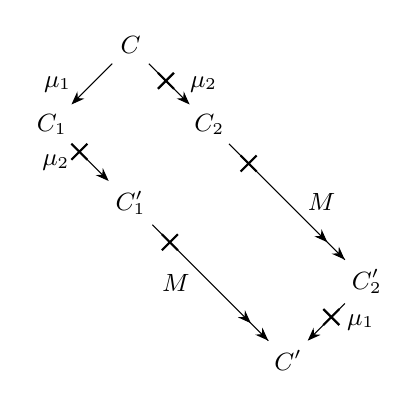
\begin{tikzpicture}[x=1cm,y=1cm, every node/.style={font=\small}]
  %--- Nodes placed to mimic the photo ----------------------------------------
  \node (C)   at (0,0) {$C$};
  \node (C2)  at (1,-1) {$C_2$};
  \node (C2p) at (3,-3) {$C_2'$};
  \node (C1)  at (-1, -1) {$C_1$};
  \node (C1p) at (0,-2) {$C_1'$};
  \node (Cp)  at (2,-4) {$C'$};

  %--- Top/right branch --------------------------------------------------------
  \draw[->] (C) -- node[right=4pt] {$\mu_2$} (C2);
  \node[cross out,draw,thick,minimum size=5pt,inner sep=0pt]
       at ($(C)!0.45!(C2)$) {};

  \draw[->] (C) -- node[left=4pt] {$\mu_1$} (C1);

  \draw[->] (C1) -- node[left=4pt] {$\mu_2$} (C1p);
  \node[cross out,draw,thick,minimum size=5pt,inner sep=0pt]
       at ($(C1)!0.35!(C1p)$) {};

  \draw[markarrows] (C2) -- node[right=4pt] {$M$} (C2p);
  \node[cross out,draw,thick,minimum size=5pt,inner sep=0pt]
       at ($(C2)!0.25!(C2p)$) {};

  \draw[markarrows] (C1p) -- node[left=4pt] {$M$} (Cp);
  \node[cross out,draw,thick,minimum size=5pt,inner sep=0pt]
       at ($(C1p)!0.25!(Cp)$) {};

  \draw[->] (C2p) -- node[right=4pt] {$\mu_1$} (Cp);
  \node[cross out,draw,thick,minimum size=5pt,inner sep=0pt]
       at ($(C2p)!0.45!(Cp)$) {};

\end{tikzpicture}
\end{wrapfigure}

While a full proof of completeness of the deterministic semantics is not given, the following diagram gives the intuition: $C$ is able to do a step in the reference semantics and reach a $C_1$ configuration, while in the deterministic semantics (denoted with the crossed arrow) $C$ reaches a \emph{different} $C_2$.
Assuming the computation from $C$ as terminating in the reference semantics, it is always reachable a common configuration $C'$ from both $C_1$ and $C_2$ using the deterministic semantics. Moreover no maximal computation can end with a non deterministic transition, so it's always possible to \emph{close} the depicted diagram.

The new semantics is deterministic as defined above: any configuration that admits an execution step admits just one, completely specified by the first instruction of the choreography. From now the deterministic semantics will be the semantics considered for \textbf{Chor}.

\subsubsection{Removal of irrelevant terms}
We want to prove that terms not present in the image of $\lfloor \cdot \rfloor$ are not relevant to natural semantics, making us able to use freely the $\lceil \cdot \rceil$ operator. We introduce the operator $\wr C \wr$ defined by structural recursion on $C$ as follows:
\begin{align*}
	\wr~\boldsymbol{0}~\wr &\triangleq \boldsymbol{0} \\
	\wr~p.e \rightarrow q.x;~ C'~\wr &\triangleq p.e \rightarrow q.x;~ \wr C' \wr \\
	\wr~p \rightarrow q[L];~ C'~\wr &\triangleq \wr C' \wr \\
	\wr~p.x := e;~ C'~\wr &\triangleq p.x := e;~ \wr C' \wr \\
	\wr~\text{if } p.e \text{ then } C_1 \text{ else } C_2;~ C'~\wr &\triangleq \text{if } p.e \text{ then } \wr C_1\wr \text{ else } \wr C_2\wr ;~ \wr C'\wr \\
	\wr~X(\vec{p}~);~ C'~\wr &\triangleq X(\vec{p}~);~ \wr C' \wr \\
	\wr~q : X(\vec{p}~).C;~ C'~\wr &\triangleq \wr C' \wr \\
\end{align*}
It is easy to verify how, for any $C$, $\lceil \wr C \wr \rceil$ is well-defined as by definition \ref{defs:lift_chor}.

We extend the operator $\wr \cdot \wr$ on \emph{procedure context}, as follows:
$$
\wr\mathscr{C}\wr \triangleq
\{X(\vec{p}) = \wr C \wr \mid X(\vec{p}) = C \in \mathscr{C}\}
$$

We now prove that this operator is complete with respect to the semantics: for each $C$ such that
$$
\langle C, \Sigma, \mathscr{C} \rangle \Downarrow^M \Sigma'
$$

There exists $M^*$ such that:
\begin{equation}
\label{aux:compl_wr}
	\langle \wr C \wr, \Sigma, \wr\mathscr{C}\wr \rangle \Downarrow^{M^*} \Sigma'
\end{equation}

\noindent \textbf{Proof:}\\
We proceed by induction on the size of $M$
\begin{itemize}
	\item \emph{size: 0} In this case the $C = \boldsymbol{0}$ and by definition
		$\wr C \wr = \boldsymbol{0}$, thus the conclusion holds.
	\item \emph{size: n+1} In this case we have two hypothesis:
		\begin{align}
			\langle C, \Sigma, \mathscr{C} \rangle& \xrightarrow{\mu}
			\langle C', \Sigma', \mathscr{C} \rangle& \tag{H1} \label{aux:compl_wr_h1}\\
			\exists M',~\langle \wr C'\wr, \Sigma', \wr \mathscr{C} \wr \rangle& \Downarrow^{M'} \Sigma'' \tag{IH} \label{aux:compl_wr_ih}
		\end{align}
		By inversion of (\ref{aux:compl_wr_h1}) we find that $C = I; C^\star$, we proceed by cases on the structure of $I$:
		\begin{itemize}
			\item \emph{assign, communication}: By further inversion of (\ref{aux:compl_wr_h1}) we find $C^\star = C'$.\\
			We now find:
			$$\wr C \wr = \wr I; C^\star \wr = \wr I; C' \wr = I;~\wr C' \wr$$
				Using (\ref{aux:compl_wr_ih}) we construct $M^* = \mu :: M'$
			\item \emph{selection, runtime term}:
				By further inversion of (\ref{aux:compl_wr_h1}) we find $C^\star = C'$ and $\Sigma = \Sigma'$.\\
			We now find:
			$$\wr C \wr = \wr I; C^\star \wr = \wr I; C' \wr = \wr C' \wr$$
				Using (\ref{aux:compl_wr_ih}) we construct $M^* = M'$
			\item \emph{function call}: By further inversion of (\ref{aux:compl_wr_h1}) we find $X(\vec{p}) = C_X \in \mathscr{C}$, $C' = p_2 : X(\vec{p}~).C^\star; \ldots; p_n : X(\vec{p}~).C^\star; C_X[\vec{q}/\vec{p}~] \fatsemi C^\star$ and $\Sigma = \Sigma'$\\
			We now find:
				$$\wr C \wr = \wr X(\vec{p}); C^\star \wr = X(\vec{p}); \wr C^\star \wr$$
			Which can do a $\mu$ step of the operational semantics and reach:
				$$p_2 : X(\vec{p}~).C^\star; \ldots; p_n : X(\vec{p}~).C^\star; \wr C_X\wr[\vec{q}/\vec{p}~] \fatsemi \wr C^\star \wr$$
			Which can do $n-1$ steps $\tau@p_2, \ldots, \tau@p_n$ and reach
				$$\wr C_X\wr[\vec{q}/\vec{p}~] \fatsemi \wr C^\star \wr$$
				We now look at $C'$ and notice, by reasoning on the definition of \emph{sequential composition} and \emph{process substitution} (proven in Appendix \ref{appdix:A}):
				\begin{align*}
					\wr C' \wr &= \wr p_2 : X(\vec{p}~).C^\star; \ldots; p_n : X(\vec{p}~).C^\star; C_X[\vec{q}/\vec{p}~] \fatsemi C^\star \wr \\
					&= \wr C_X[\vec{q}/\vec{p}~] \fatsemi C^\star \wr =
		\wr C_X[\vec{q}/\vec{p}~] \wr \fatsemi \wr C^\star \wr =
				\wr C_X\wr[\vec{q}/\vec{p}~] \fatsemi \wr C^\star \wr
				\end{align*}
				Using (\ref{aux:compl_wr_ih}) we construct
				$$ M^* = \mu :: \tau@p_2 :: \ldots :: \tau@p_n :: M'$$
			\item \emph{conditional} (for brevity we will only consider the \emph{true} case, the other one follows by symmetry):
				By further inversion of (\ref{aux:compl_wr_h1}) we find $C' = C_1 \fatsemi C^\star$ and $\Sigma = \Sigma'$.\\
				We now find:
				$$
				\wr C \wr = \wr~\text{if } p.e \text{ then } C_1 \text{ else } C_2;~C^\star~\wr 
				= \text{if } p.e \text{ then } \wr C_1 \wr \text{ else } \wr C_2\wr;~\wr C^\star \wr 
				$$
				Which can do a $\mu$ step and reach:
				$$ \wr C_1 \wr \fatsemi \wr C^\star \wr = \wr C_1 \fatsemi C^\star \wr = \wr C' \wr$$
				Using (\ref{aux:compl_wr_ih}) we construct $M^* = \mu :: M'$
		\end{itemize}
\end{itemize}
$\qed$

\subsubsection{Ramifications on the semantic for procedure calls}
Since, as we saw in the previous section, \emph{runtime terms} are irrelevant for the computation, we will now change the semantics for CALL-FIRST to the following rule, which also makes CALL-ENTER unreachable:
$$
    \inferrule*[right=call] { X(\vec{q}~) = C \in \mathscr{C}}
	{\langle X(\vec{p}~);C', \Sigma, \mathscr{C} \rangle \xrightarrow{\cdot} \langle C[\vec{q}/\vec{p}~] \fatsemi C', \Sigma, \mathscr{C} \rangle}
$$
The correctness of this change follows from the previous proof: since both rules have as result $\wr$-equivalent configurations (we will omit a formal discussion of this equivalence) the state reached by the computation is unchanged.\\
The justification for not specifying the transition label associated with the inference rule is that we are going to mostly ignore the transition labels from now on.

\subsubsection{Completeness of the instrumented semantics}
We take a  $C, \mathscr{C}$ for which $\lceil \cdot \rceil$ is well defined.
We have to prove that, given:
$$
\langle C, \lfloor \Sigma \rfloor, \mathscr{C}\rangle \Downarrow^M \Sigma'
$$
then there exists $\Sigma''$ such that:
$$
\langle \lceil C \rceil, \Sigma, \lceil \mathscr{C}\rceil\rangle \Downarrow \Sigma''
\land \Sigma' = \lfloor \Sigma'' \rfloor 
$$


\noindent\textbf{Proof:}\\
We proceed by induction of the size of $\cdot \Downarrow^M \cdot$:
\begin{itemize}
\item \emph{size: 0}: We have 
$$ C = \boldsymbol{0} = \lceil C \rceil
\quad \text{and}\quad \lfloor \Sigma \rfloor = \Sigma'$$
so the conclusion follows with $\Sigma'' = \Sigma$
\item \emph{size: n + 1}: We have the following hypothesis:
\begin{align}
&\langle C, \lfloor \Sigma \rfloor, \mathscr{C}\rangle \xrightarrow{.}
\langle C^\star, \Sigma^\star, \mathscr{C}\rangle
\label{aux:comp_h1}\tag{H1}\\
&\langle C^\star, \Sigma^\star, \mathscr{C}\rangle
\Downarrow^\cdot \Sigma'
\label{aux:comp_h2}\tag{H2}\\
&\forall~\Sigma^\heart, \lfloor \Sigma^\heart \rfloor = \Sigma^\star
\Rightarrow \langle \lceil C^\star \rceil, \Sigma^\heart, \lceil \mathscr{C} \rceil\rangle \Downarrow \Sigma'' \land \lfloor \Sigma'' \rfloor = \Sigma'
\label{aux:comp_ih}\tag{IH}
\end{align}
We proceed by inversion on (\ref{aux:comp_h1})
\begin{itemize}
\item LOCAL: Inversion gives us:
\begin{align}
&C = p.x := e;~ C^\star \label{aux:comp_ass1}\tag{I1}\\
&\lfloor \Sigma \rfloor~p \vdash e \downarrow v \label{aux:comp_ass2}\tag{I2}\\
&\Sigma^\star = \lfloor \Sigma \rfloor[p.x \mapsto v]\label{aux:comp_ass3}\tag{I3}
\end{align}
By \emph{correctness} of the local evaluation (\ref{inst:loc_correct}) and (\ref{aux:comp_ass2}) we find:
\begin{equation}\label{aux:comp_ass4}
\Sigma~p \vdash e \downarrow [v] \quad \lor \quad
\Sigma~p \vdash e \downarrow v
\end{equation}
We proceed by cases on the hypothesis:
\begin{itemize}
\item \emph{case left:}
By definition of $\lceil \cdot \rceil$ we have:
$$\lceil C \rceil = p.x := e;~\lceil C^\star \rceil$$
We do the following execution steps:
\begin{align*}
&\langle p.x := e;~\lceil C^\star \rceil, \Sigma, \lceil \mathscr{C}\rceil\rangle\\
&\rightarrow\langle \boldsymbol{0};~\lceil C^\star \rceil, \Sigma[p.x \mapsto [v]], \lceil \mathscr{C} \rceil \rangle\\
&\rightarrow\langle \lceil C^\star \rceil, \Sigma[p.x \mapsto [v]], \lceil \mathscr{C} \rceil \rangle
\end{align*}
From which, using the fact that (equivalences on syntactic transformations are proved in Appendix \ref{appdix:A})
$$
		\lfloor\Sigma^\heart\rfloor = \lfloor \Sigma[p.x \mapsto [v]] \rfloor = \lfloor \Sigma \rfloor[p.x \mapsto v] = \Sigma^\star
$$
We can use the induction hypothesis (\ref{aux:comp_ih})
\item \emph{case right:} We have two possible rules regarding assignment with (\ref{aux:comp_ass4}) as antecedent, depending on the value of $\Gamma~p~x$. We proceed by \emph{law of excluded middle} and find:
\begin{equation}\label{aux:comp_ass5}
\Gamma~p~x \not\sqsubseteq low \quad \lor \quad
\Gamma~p~x \sqsubseteq low
\end{equation}
In the \emph{left case} we proceed exactly as the previously specified proof case, adjusting the inference rule used for the first step. In the \emph{right case} we follow similarly, with the only difference being:
$$
\Sigma^\heart = \Sigma[p.x\mapsto v]
$$
\end{itemize}
\item COM: The inductive case follows similarly to the LOCAL one, substituting $p.x$ with $q.x$ when needed.
\item COND-THEN: Inversion gives us:
\begin{align}
&C = \text{if } p.e \text{ then } C_1 \text{ else } C_2;~ C' \label{aux:comp_then1}\tag{I1}\\
	&C^\star = C_1 \fatsemi C'\label{aux:comp_then2}\tag{I2}\\
&\lfloor \Sigma \rfloor~p \vdash e \downarrow true \label{aux:comp_then3}\tag{I3}\\
&\Sigma^\star = \lfloor \Sigma \rfloor\label{aux:comp_then4}\tag{I4}
\end{align}
By definition of $\lceil \cdot \rceil$ we have:
$$
\lceil C\rceil = \text{if } p.e \text{ then } \lceil C_1\rceil \text{ else }\lceil C_2\rceil;~ \lceil C'\rceil
$$
We use lemma (\ref{appdix:Bfat}) on (\ref{aux:comp_ih}) and find:
$$
\langle \lceil C_1 \rceil, \Sigma, \lceil \mathscr{C} \rceil \rangle \twoheadrightarrow \langle \boldsymbol{0}, \Sigma^\dag, \lceil \mathscr{C} \rceil \rangle 
\land
\langle \lceil C' \rceil, \Sigma^\dag, \lceil \mathscr{C} \rceil \rangle \Downarrow \Sigma''
$$
Which let's us construct the following computation:
\begin{align*}
&\langle \text{if } p.e \text{ then } \lceil C_1\rceil \text{ else }\lceil C_2\rceil;~ \lceil C'\rceil, \Sigma, \lceil \mathscr{C}\rceil\rangle\\
&\rightarrow \langle \lceil C_1\rceil;~ \lceil C'\rceil, \Sigma, \lceil \mathscr{C}\rceil\rangle\\
&\twoheadrightarrow \langle \boldsymbol{0};~ \lceil C'\rceil, \Sigma^\dag, \lceil \mathscr{C} \rceil \rangle \\
&\rightarrow \langle \lceil C'\rceil, \Sigma^\dag, \lceil \mathscr{C} \rceil \rangle\Downarrow \Sigma''
\end{align*}
\item COND-ELSE: This inductive step is symmetric with respect to COND-THEN
\item CALL: Inversion gives us:
\begin{align}
&C = X(\vec{p});~ C' \label{aux:comp_call1}\tag{I1}\\
&X(\vec{q}) = C_X \in \mathscr{C} \label{aux:comp_call2}\tag{I2}\\
&C^\star = C_X[\vec{q}/\vec{p}] \fatsemi C'\label{aux:comp_then3}\tag{I3}\\
&\Sigma^\star = \lfloor \Sigma \rfloor\label{aux:comp_then4}\tag{I4}
\end{align}
By definition of $\lceil \cdot \rceil$ we have:
$$
\lceil C\rceil = X(\vec{p});~ \lceil C'\rceil
$$
We use lemma (\ref{appdix:Bfat}) on (\ref{aux:comp_ih}) and find:
$$
\langle \lceil C_X[\vec{p}/\vec{q}] \rceil, \Sigma, \lceil \mathscr{C} \rceil \rangle \twoheadrightarrow \langle \boldsymbol{0}, \Sigma^\dag, \lceil \mathscr{C} \rceil \rangle 
\land
\langle \lceil C' \rceil, \Sigma^\dag, \lceil \mathscr{C} \rceil \rangle \Downarrow \Sigma''
$$
By definition of $\lceil \mathscr{C} \rceil$, then:
$$
X(\vec{q}) = \lceil C_X \rceil \in \lceil \mathscr{C} \rceil
$$
Which let's us construct the following computation (equivalences on syntactic transformations are proved in Appendix \ref{appdix:A}):
\begin{align*}
&\langle X(\vec{p});~ \lceil C'\rceil, \Sigma, \lceil \mathscr{C}\rceil\rangle\\
&\rightarrow \langle \lceil C_X\rceil[\vec{q}/\vec{p}];~ \lceil C'\rceil, \Sigma, \lceil \mathscr{C}\rceil\rangle\\
&= \langle \lceil C_X[\vec{q}/\vec{p}]\rceil;~ \lceil C'\rceil, \Sigma, \lceil \mathscr{C}\rceil\rangle\\
&\twoheadrightarrow \langle \boldsymbol{0};~ \lceil C'\rceil, \Sigma^\dag, \lceil \mathscr{C} \rceil \rangle \\
&\rightarrow \langle \lceil C'\rceil, \Sigma^\dag, \lceil \mathscr{C} \rceil \rangle\Downarrow \Sigma''
\end{align*}
\end{itemize}
\end{itemize}
$\qed$

\subsubsection{Putting all the steps together}
We saw how, starting from a maximal computation
$$\langle C, \Sigma, \mathscr{C}\rangle \Downarrow^M \Sigma'$$
We can:
\begin{itemize}
\item Replace every non-deterministic aspect of the computation without changing the result, thus letting us reason only on the deterministic subset of the semantics.
\item Remove terms which do not affect the computation result, thus letting us ignore them.
\item Construct a computation in the instrumented semantics that maintains $low$-equivalence for stores.
\end{itemize}
Thus, since by definition:
$$ \lfloor \lceil \Sigma \rceil^\Gamma \rfloor = \Sigma $$
Then the \emph{completeness lemma} as stated in (\ref{aux:compl}) is proven. $\qed$


\subsection{Completeness of type extension}\label{aux:ext_tj}
This lemma tells us that \emph{lifting} a choreography maintains typing.\\
Formally:
$$
\Delta;\Gamma;\bot \vdash C \Rightarrow
\Delta;\Gamma;\bot \vdash \lceil \wr C \wr \rceil
$$

\noindent\textbf{Proof:}\\
The type judgment is clearly maintained by $\wr \cdot \wr$ because the only effect of the operator is to \emph{remove} instructions.
The following is a more general case easy to verify by inverting the typing rule for sequences (which is basically a \emph{conjunction}):
$$
\Delta;\Gamma;\bot \vdash I;C \Rightarrow \Delta;\Gamma;\bot \vdash C
$$
We can verify that \emph{lifting} maintains typing by noticing that $\lceil C \rceil$ never introduces a \emph{bracketed} term and for any non bracketed term the typing rules are syntactically equivalent between \textbf{Chor} and \textbf{[Chor]}.
$\qed$

\subsection{Preservation lemma}
The preservation lemma (i.e. subject reduction) states that the operational semantics preserves typing, that is \emph{starting from a well typed configuration executing a step of the semantics gives you a well typed configuration}.
We are now working only in the instrumented semantics, thus we will omit the redundant brackets when sufficiently clear.\\
A configuration
$\langle C, \Sigma, \mathscr{C}\rangle$ is well-typed for a $pc \in \MCL$ when:
$$\Delta, \Gamma, pc \vdash C \quad \text{and}\quad \Gamma \vdash \Sigma$$
The preservation lemma is stated as follows:
\begin{equation}\label{aux:pres}
\Delta, \Gamma, pc \vdash C \land \Gamma \vdash \Sigma \land 
\langle C, \Sigma, \mathscr{C}\rangle \rightarrow
\langle C', \Sigma', \mathscr{C}\rangle \Rightarrow 
\Delta, \Gamma, pc \vdash C' \land \Gamma \vdash \Sigma'
\end{equation}
It is easy to see how the preservation lemma can be easily carried over to $\cdot \twoheadrightarrow \cdot$.

\medskip
\noindent\textbf{Proof:}\\
The majority of the preservation proof follows directly from \cite{myers2011proving} thus we will explain only the part which differ.\\
The main difference between our instrumented syntax and the language presented in \cite{myers2011proving} is the presence of recursive procedures.

The inductive case that we have to consider is:
\begin{align}
	&\Delta,\Gamma,pc \vdash X(\vec{p})\label{aux:pres_Htj}\tag{H1}\\
	&\langle X(\vec{p}), \Sigma, \mathscr{C}\rangle \rightarrow
	\langle C_X[\vec{q}/\vec{p}], \Sigma, \mathscr{C}\rangle\label{aux:pres_Hlto}\tag{H2}\\
	&X(\vec{q}) = C_X \in \mathscr{C}\label{aux:pres_Hlook}\tag{H3}
\end{align}
By inversion on (\ref{aux:pres_Htj}) we find:
\begin{align}
	&\Gamma' \in \Delta(X,pc) \label{aux:pres_Htj1}\tag{H11}\\
	&\Gamma[\vec{q}\mapsto \vec{p}] \equiv_{\{\vec{q}\}} \Gamma'\label{aux:pres_Htj2}\tag{H12}
\end{align}
By definition of $\Delta$, then
$$
\Gamma' \in \Delta(X,pc) \Rightarrow \Delta, \Gamma', pc \vdash C_X
$$
We now state a lemma which will not be proven in this document (since it is quite long and syntactical), but is part of the \emph{lean} artifact.
\begin{align*}\label{aux:pres_lemma2}
\begin{split}
	\Delta, \Gamma', pc \vdash C 
	&\Rightarrow~ pn(C) \subseteq \vec{q}\\
	\Rightarrow~ \Gamma'' \equiv_{\{\vec{q}\}} \Gamma'
	&\Rightarrow~ \Delta, \Gamma'', pc \vdash C
\end{split}
\end{align*}

From \emph{well-formedness of procedure context} (assumed in \ref{ass:wellf_ctx})
we know that $pn(C_X) \subseteq \vec{q}$ thus we find
$$
\Delta,\Gamma[\vec{q}\mapsto\vec{p}],pc \vdash C_X
$$

We now introduce another lemma, proven in the \emph{lean} code but for which the proof (for the same reasons as above) will not be reproduced in this document.

\begin{equation*}\label{aux:pres_lemma1}
\Delta, \Gamma[\vec{q}\mapsto\vec{p}], pc \vdash C \Rightarrow
\Delta, \Gamma, pc \vdash C[\vec{q}/\vec{p}]
\end{equation*}
This lemma requires \emph{freshness of formal parameters} to be proven, assumed in \ref{ass:fresh}.
We now remind ourselves the conclusion to be proven, that is:
$$
\Delta, \Gamma, pc \vdash C_X[\vec{q}/\vec{p}]\quad\land\quad \Gamma \vdash \Sigma
$$
The left-hand side is proven by the previous chain of steps.
The right-hand side is easy to prove from hypothesis of the preservation lemma.
$\qed$

\paragraph{pc subsumption:}
Subsumption of procedures invocation (used in the proof in \cite{myers2011proving} for conditional steps) is directly given by the assumption in \ref{ass:ctx_sub}

\subsection{Unwinding lemma}
The unwinding lemma states that the operational semantics preserves low-equal configurations. We formalize this as follows:\\
Given well-typed $C_1~C_2$ in \textbf{[Chor]}, well-formed $\Sigma_1, \Sigma_2$ is \textbf{[CStore]} then:
$$
C_1 \approx_{low} C_2 \land
\Sigma_1 \approx_{low} \Sigma_2 \land
\langle C_1, \Sigma_1, \mathscr{C} \rangle \rightarrow
\langle C_1', \Sigma_1', \mathscr{C} \rangle
$$
implies that there either exists $C_2'~\Sigma_2'$ s.t.
\begin{equation}\label{aux:unw}
\langle C_2, \Sigma_2, \mathscr{C} \rangle \twoheadrightarrow
\langle C_2', \Sigma_2', \mathscr{C} \rangle
\land C_1' \approx_{low} C_2'
\land \Sigma_1' \approx_{low} \Sigma_2'
\end{equation}
or that $\langle C_2, \Sigma_2, \mathscr{C}\rangle$ diverges.

The proof of this lemma is mostly unchanged from the one presented in \cite{myers2011proving} since the differences between the two languages treated are not relevant. For this reason, we omit the proof from this document.

\section{Main proof}
We remind ourselves the main theorem as stated in (\ref{main:def}):
\begin{align*}
	&\Delta;\Gamma;\bot \vdash C \Rightarrow
	\Sigma_1 \equiv^\Gamma_{low} \Sigma_2 \\ \Rightarrow\ &\langle C, \Sigma_1, \mathscr{C}\rangle \Downarrow^{M_1} \Sigma'_1
	\Rightarrow\ \langle C, \Sigma_2, \mathscr{C}\rangle \Downarrow^{M_2} \Sigma'_2 \\ \Rightarrow\ &\Sigma'_1 \equiv^\Gamma_{low} \Sigma'_2
\end{align*}

\noindent\textbf{Proof:}\\
By completeness (\ref{aux:compl}) we find:
$$
	\langle \lceil \wr C \wr \rceil, \lceil \Sigma_1 \rceil^\Gamma, \lceil \mathscr{C}\rceil \rangle \Downarrow [\Sigma]'_1 \quad \text{and} \quad
	\langle \lceil \wr C \wr \rceil, \lceil \Sigma_2 \rceil^\Gamma, \lceil \mathscr{C}\rceil\rangle \Downarrow [\Sigma]'_2
$$
such that
\begin{equation}\label{main:low_eq_cs}
\lfloor [\Sigma]'_1 \rfloor = \Sigma'_1 \quad \text{and} \quad
\lfloor [\Sigma]'_2 \rfloor = \Sigma'_2
\end{equation}
By extension of typing (\ref{aux:ext_tj}) we have:
$$\Delta;\Gamma;\bot \vdash \lceil \wr C \wr \rceil$$
By definition of $\lceil \cdot \rceil^\Gamma$ we have
$$
i \in {1,2} \quad \lceil \Sigma_i \rceil^\Gamma \Rightarrow
\Gamma \vdash \lceil \Sigma_i \rceil^\Gamma
$$
We can thus use preservation (\ref{aux:pres}) to find
$$
\Gamma \vdash [\Sigma]_1' \quad \text{and} \quad \Gamma \vdash [\Sigma]_2'
$$
That, with (\ref{main:low_eq_cs}) let's us reduce the proof of $
\Sigma_1' \equiv_{low}^\Gamma \Sigma_2'$ to the proof of
$ [\Sigma]_1' \approx_{low} [\Sigma]_2' $

\bigskip
\noindent We have now reduced the proof to the following:
\begin{align*}
	&\Delta;\Gamma;\bot \vdash \lceil \wr C \wr \rceil \\
	\Rightarrow\ &\langle \lceil \wr C \wr \rceil, \lceil \Sigma_1 \rceil^\Gamma, \lceil \mathscr{C} \rceil\rangle \Downarrow [\Sigma]'_1 \\
	\Rightarrow\ &\langle \lceil \wr C \wr \rceil, \lceil \Sigma_2 \rceil^\Gamma, \lceil \mathscr{C} \rceil\rangle \Downarrow [\Sigma]'_2 \\
	\Rightarrow\ &[\Sigma]'_1 \approx_{low} [\Sigma]'_2
\end{align*}
By $\Sigma_1 \equiv^\Gamma_{low} \Sigma_2$ and well-formedness of the contexts we have
$$
\lceil \Sigma_1 \rceil^\Gamma \approx_{low} \lceil \Sigma_2 \rceil^\Gamma
$$
By reflexivity of $\approx_{low}$ we have
$$
\lceil \wr C \wr \rceil \approx_{low} \lceil \wr C \wr \rceil
$$
We generalize over the specific construction of
$ \lceil \Sigma_1 \rceil^\Gamma,~\lceil \Sigma_2 \rceil^\Gamma,~\lceil \wr C \wr \rceil $ and just keep the previously stated low-equivalences between them.
At this point the proof follows by induction on the size of $\langle \cdot, \cdot, \cdot\rangle \Downarrow [\Sigma]_1'$:
\begin{itemize}
	\item \emph{size 0}: Transition of size zero means that the first choreography is $\boldsymbol{0}$. By definition of $\approx_{low}$ the second is $\boldsymbol{0}$ as-well. By hypothesis the two $\Sigma$ are equivalent, thus the conclusion follows
	\item \emph{size n+1}: This means that the first transition is composed by at least one step of the operational semantics:
$$
		\langle [C]_1, [\Sigma]_1, \lceil\mathscr{C}\rceil\rangle \rightarrow
		\langle [C]_1^*, [\Sigma]_1^*, \lceil\mathscr{C}\rceil\rangle
$$
		By unwinding (\ref{aux:unw}) we find $[C_2]^*,~[\Sigma]_2^*$ s.t. the low-equivalence is respected (since we are proving \emph{TINI} we have as hypothesis that the computation from $\langle [C]_2, [\Sigma]_2, \lceil\mathscr{C}\rceil\rangle$ does not diverge).
		By preservation (\ref{aux:pres}) we find well-typedness and well-formedness needed to use the induction hypothesis, from which we prove the conclusion.
\end{itemize}
$\qed$

\begin{appendices}
\chapter{Proofs on syntactic transformations}
\label{appdix:A}
\section{Sequential composition and $\wr \cdot \wr$}
We need to prove the following:
$$\wr C_1 \fatsemi C_2 \wr = \wr C_1 \wr \fatsemi \wr C_2 \wr$$

\noindent\textbf{Proof:}
This proof follows by induction on $C_1$, unrolling the definitions of the operators involved.

\section{Process substitution and $\wr \cdot \wr$}
We need to prove the following:
$$\wr C [\vec{q}/\vec{p}] \wr = \wr C \wr [\vec{q}/\vec{p}]$$

\noindent\textbf{Proof:}
This proof follows by induction on $C$, unrolling the definitions of the operators involved.

\section{Store update and $\lfloor \cdot \rfloor$}
We need to prove the following:
$$\lfloor \Sigma \rfloor[p.x \mapsto v] = \lfloor \Sigma[p.x \mapsto [v]] \rfloor$$

\noindent\textbf{Proof:}
We defined equivalence between stores as extensional equivalence between maps.
This theorem follows from triangular reasoning:\\
For $q.y$ different from $p.x$:
\begin{align*}
&\lfloor \Sigma \rfloor[p.x \mapsto v]~q.y = \lfloor \Sigma \rfloor~q.y\\
&\lfloor \Sigma [p.x \mapsto [v]] \rfloor~q.y = \lfloor \Sigma \rfloor~q.y
\end{align*}
While simultaneously:
\begin{align*}
&\lfloor \Sigma \rfloor[p.x \mapsto v]~p.x = v\\
&\lfloor \Sigma [p.x \mapsto [v]] \rfloor~p.x = \lfloor [v] \rfloor = v
\end{align*}


\section{Process substitution and $\lceil \cdot \rceil$}
We need to prove the following:
$$\wr C [\vec{q}/\vec{p}] \wr = \wr C \wr [\vec{q}/\vec{p}]$$

\noindent\textbf{Proof:}
This proof follows by induction on $C$, unrolling the definitions of the operators involved.


\chapter{Decomposition of sequential composition execution}
\label{appdix:B}
\section{\textbf{[Chor]} Sequential composition}
We start by proving the following lemma:
\begin{align}
\begin{split}
\label{appdix:Bskin}
&\langle C_1 ; C_2, \Sigma, \mathscr{C}\rangle \Downarrow \Sigma''\\
&\Rightarrow \exists \Sigma',
\langle C_1, \Sigma, \mathscr{C} \rangle \twoheadrightarrow \langle \boldsymbol{0}, \Sigma', \mathscr{C} \rangle 
\quad\land\quad
\langle C_2, \Sigma', \mathscr{C} \rangle \Downarrow \Sigma''
\end{split}
\end{align}

\noindent\textbf{Proof:}
We proceed by induction on $\cdot \Downarrow \cdot$
\begin{itemize}
\item \emph{case nil:} This case is not possible because there are no $C_1, C_2$ such that $\boldsymbol{0} = C_1; C_2$. Thus the goal follows by \emph{ex-falso quodlibet}.
\item \emph{case step:} the inductive case gives us the following hypothesis:
\begin{align}
&\langle C_1; C_2, \Sigma, \mathscr{C}\rangle \rightarrow
\langle C^\star, \Sigma^\star, \mathscr{C}\rangle \label{appdix:b1_h1} \tag{H1}\\
\begin{split}
&\forall C_1^\star~C_2^\star,\quad C^\star = C_1^\star; C_2^\star \\
&\Rightarrow \exists \Sigma^\heart,~\langle C_1^\star, \Sigma^\star, \mathscr{C}\rangle \rightarrow \langle \boldsymbol{0}, \Sigma^\heart, \mathscr{C}\rangle ~\land~ \langle C_2^\star, \Sigma^\heart, \mathscr{C}\rangle \Downarrow \Sigma'' \\
\end{split}\label{appdix:b1_ih}\tag{IH}
\end{align}
By inversion on (\ref{appdix:b1_h1}) we find two possible cases:
\begin{itemize}
\item $\langle C_1, \Sigma, \mathscr{C}\rangle \rightarrow
\langle C_1^\star, \Sigma^\star, \mathscr{C}\rangle$ with $C^\star = C_1^\star; C_2$
\item $\langle \boldsymbol{0}; C_2, \Sigma, \mathscr{C}\rangle \rightarrow
\langle C_2, \Sigma^\star, \mathscr{C}\rangle$ thus with $C^\star = C_2$
\end{itemize}
Both cases follow easily from the previous hypothesis. $\qed$
\end{itemize}


\section{\textbf{Chor} Sequential composition}
We finally to prove the following statement:
\begin{align}
\begin{split}
\label{appdix:Bfat}
&\langle \lceil C_1 \fatsemi C_2\rceil, \Sigma, \mathscr{C}\rangle \Downarrow \Sigma''\\
&\Rightarrow \exists \Sigma',
\langle \lceil C_1 \rceil, \Sigma, \mathscr{C} \rangle \twoheadrightarrow \langle \boldsymbol{0}, \Sigma', \mathscr{C} \rangle 
\quad\land\quad
\langle \lceil C_2 \rceil, \Sigma', \mathscr{C} \rangle \Downarrow \Sigma''
\end{split}
\end{align}

\noindent\textbf{Proof:}
We proceed by induction on $C_1$:
\begin{itemize}
\item \emph{case $\boldsymbol{0}$:} by definition of $\cdot \fatsemi \cdot$ we have that:
$$
\lceil C_1 \fatsemi C_2 \rceil = \lceil C_2 \rceil
$$
And the conclusion follows by reflexivity of $\cdot \twoheadrightarrow \cdot$, with $\Sigma' = \Sigma$
\item \emph{case $I_1; C_1'$:} As \emph{induction hypothesis} we have that, for all $\Sigma^\heart$
\begin{align*}
\begin{split}
\langle \lceil C_1' \fatsemi C_2\rceil, \Sigma^\heart, \mathscr{C}\rangle \Downarrow \Sigma''
\Rightarrow \exists \Sigma^\star,
\langle \lceil C_1' \rceil, \Sigma^\heart, \mathscr{C} \rangle \twoheadrightarrow \langle \boldsymbol{0}, \Sigma^\star, \mathscr{C} \rangle 
\quad\land\quad
\langle \lceil C_2 \rceil, \Sigma^\star, \mathscr{C} \rangle \Downarrow \Sigma''
\end{split}
\end{align*}
By definition of $\lceil \cdot \rceil, \cdot \fatsemi \cdot$ we have:
$$
\lceil C_1 \fatsemi C_2 \rceil = \lceil (I_1; C_1') \fatsemi C_2 \rceil =
\lceil I_1; (C_1' \fatsemi C_2) \rceil = \lceil I_1 \rceil; \lceil C_1' \fatsemi C_2 \rceil
$$
\end{itemize}
Using lemma (\ref{appdix:Bskin}) we find:
$$
\exists \Sigma^\heart,~\langle \lceil I_1 \rceil, \Sigma, \mathscr{C} \rangle \twoheadrightarrow \langle \boldsymbol{0}, \Sigma^\heart, \mathscr{C} \rangle ~\land~ \langle \lceil C_1' \fatsemi C_2 \rceil, \Sigma^\heart, \mathscr{C}\rangle \Downarrow \Sigma''
$$
Thus we prove the goal by choosing $\Sigma' = \Sigma^\star$ and constructing the following execution (the extension of the semantics rule for $\cdot;\cdot$ to $\cdot \twoheadrightarrow \cdot$ is assumed as obvious):
\begin{align*}
\langle \lceil I_1\rceil; \lceil C_1'\rceil, \Sigma, \mathscr{C}\rangle
&\twoheadrightarrow
\langle \boldsymbol{0}; \lceil C_1'\rceil, \Sigma^\heart, \mathscr{C}\rangle\\
\rightarrow \langle \lceil C_1' \rceil, \Sigma^\heart, \mathscr{C}\rangle
&\twoheadrightarrow \langle \boldsymbol{0}, \Sigma^\star, \mathscr{C}\rangle\\
	\land\quad \langle\lceil C_2 \rceil, \Sigma^\star,\mathscr{C}\rangle \Downarrow \Sigma''&
\end{align*}
$\qed$

\end{appendices}


\bibliographystyle{plain}
\bibliography{refs}

\chapter*{Acknowledgments}
Thank you all
\end{document}
